% Laporan Milestone 2 — IF4031 Arsitektur Aplikasi Terdistribusi — Kelompok IMade
% Kompilasi: latexmk -pdf IF4031_M2_IMade.tex   (atau pdflatex dua kali)
% Penanda \isi{...} (merah) = bagian yang masih harus diisi; \tinjau{...} (oranye) = perlu ditinjau pemilik bagian.
\documentclass[12pt,a4paper]{article}

\usepackage[a4paper,top=2.5cm,bottom=2.5cm,left=2.5cm,right=2.5cm]{geometry}
\usepackage[T1]{fontenc}
\usepackage[utf8]{inputenc}
\usepackage{newtxtext,newtxmath}
\usepackage[indonesian]{babel}
\usepackage{setspace}
\usepackage{array,tabularx,longtable,multirow}
\usepackage{enumitem}
\usepackage{xcolor}
\usepackage{graphicx}
\usepackage{tikz}
\usetikzlibrary{arrows.meta,positioning,fit,backgrounds,calc}
\usepackage{float}
\usepackage{caption}
\usepackage{listings}
\usepackage{titlesec}
\usepackage{fancyvrb}
\usepackage[hidelinks]{hyperref}
\usepackage{url}
\def\UrlBreaks{\do\/\do-\do\_\do.}
\sloppy

\setstretch{1.15}
\setlength{\parindent}{0pt}
\setlength{\parskip}{6pt}
\renewcommand{\arraystretch}{1.25}
\setlength{\tabcolsep}{4pt}
\setlist{itemsep=2pt,topsep=4pt}

% ── Penanda isian ────────────────────────────────────────────
\newcommand{\isi}[1]{\textcolor{red}{\textbf{[ISI: #1]}}}
\newcommand{\tinjau}[1]{\textcolor{orange!80!black}{\textit{[Perlu ditinjau #1]}}}
\newcommand{\kode}[1]{\texttt{\small #1}}
\newcommand{\gambarplaceholder}[2]{%
  \begin{figure}[H]\centering
  \fbox{\parbox[c][#2][c]{0.85\textwidth}{\centering\textcolor{red}{\textbf{[GAMBAR: #1]}}}}
  \caption{#1}\end{figure}}

% ── Kode / perintah ──────────────────────────────────────────
\lstset{basicstyle=\ttfamily\footnotesize,breaklines=true,columns=fullflexible,
  frame=single,framesep=4pt,xleftmargin=6pt,xrightmargin=6pt,showstringspaces=false,
  backgroundcolor=\color{gray!6},literate={≤}{{$\le$}}1 {≥}{{$\ge$}}1 {→}{{$\rightarrow$}}1 {—}{{---}}1}

% ── Judul bab seperti laporan M1: "BAB I" + judul, di tengah ──
\titleformat{\section}[display]{\centering\bfseries\Large}{}{0pt}{}
\titleformat{\subsection}{\bfseries\normalsize}{\thesubsection.}{0.5em}{}
\titleformat{\subsubsection}{\bfseries\normalsize}{\thesubsubsection.}{0.5em}{}
\renewcommand{\thesubsection}{\arabic{subsection}}
\renewcommand{\thesubsubsection}{\alph{subsubsection}}
\newcommand{\bab}[2]{\clearpage\section*{#1\\#2}\addcontentsline{toc}{section}{#1 #2}\setcounter{subsection}{0}}
\newcommand{\bagian}[1]{\clearpage\section*{#1}\addcontentsline{toc}{section}{#1}}

% Daftar isi seperti laporan M1: entri bab tebal dengan titik pemandu
\makeatletter
\renewcommand{\l@section}[2]{\@dottedtocline{1}{0em}{0em}{\bfseries #1}{\bfseries #2}}
\renewcommand{\l@subsection}{\@dottedtocline{2}{1.5em}{1.8em}}
\makeatother
\renewcommand{\contentsname}{DAFTAR ISI}

\begin{document}

% ════════════════════════════ SAMPUL ════════════════════════════
\begin{titlepage}
\centering
\vspace*{4cm}
{\LARGE\bfseries LAPORAN MILESTONE 2\par}
{\LARGE\bfseries IF4031 Arsitektur Aplikasi Terdistribusi\par}
{\LARGE\bfseries IMade\par}
\vspace{2.5cm}
Disusun Oleh:\par\vspace{0.6cm}
Kelompok IMade\par\vspace{0.6cm}
\begin{tabular}{@{}ll@{}}
Theo Kurniady & (13523154)\\
Hasri Fayadh Muqaffa & (13523156)\\
I Made Wiweka Putera & (13523160)\\
\end{tabular}
\par\vspace{1cm}
SEKOLAH TEKNIK ELEKTRO DAN INFORMATIKA\par
INSTITUT TEKNOLOGI BANDUNG\par
SEMESTER 1 TAHUN 2026/2027\par
\end{titlepage}

% ════════════════════════════ DAFTAR ISI ════════════════════════
\begin{center}{\Large\bfseries DAFTAR ISI}\end{center}
\renewcommand{\contentsname}{}
\vspace{-1.5cm}
\tableofcontents

% ════════════════════════════ LAMPIRAN ══════════════════════════
\bagian{LAMPIRAN}

Tugas dan laporan ini disusun dengan bantuan model bahasa besar (LLM) dalam proses implementasi. Seluruh hasil yang dibantu telah ditinjau, dipahami, dan diverifikasi oleh anggota kelompok.

\vspace{1cm}
\noindent
\begin{tabular}{@{}p{0.5\textwidth}@{}p{0.5\textwidth}@{}}

\includegraphics[height=2.4cm]{gambar/ttd-fayadh.png} & 
\includegraphics[height=2.4cm]{gambar/ttd-made.png}\\
Hasri Fayadh Muqaffa (13523156) & I Made Wiweka Putera (13523160)\\[1.2cm]

\includegraphics[height=2.4cm]{gambar/ttd-theo.png} & \\
Theo Kurniady (13523154) & \\
\end{tabular}


% ════════════════════════════ BAB I ═════════════════════════════
\bab{BAB I}{Umum}

% ─────────────────────────────────────────────────────────────
\subsection{Tabel Kontribusi}

\begin{center}
\begin{tabularx}{\textwidth}{|c|p{4.2cm}|c|X|}
\hline
\textbf{No} & \textbf{Nama} & \textbf{NIM} & \textbf{Peran pada Milestone 2}\\ \hline
1 & Theo Kurniady & 13523154 & P3 inti (kebijakan skema, \textit{dead-letter queue}, \textit{replay}), P4 (Feed Satelit $\rightarrow$ WILDFIRE), Observabilitas (metrik, \textit{tracing}, dashboard)\\ \hline
2 & Hasri Fayadh Muqaffa & 13523156 & Platform Kubernetes (k3s, manifest, Secret, NetworkPolicy, \textit{one-command deploy}, Tester Agent), P2 uji beban (10.000 VU, \textit{scaling}, \textit{rolling update}), P3 laporan Tim Lapangan, P5 (Sensor Pantai, ketahanan, SLO, \textit{game day})\\ \hline
3 & I Made Wiweka Putera & 13523160 & P1 (penyimpanan terdistribusi, Audit API, dashboard analitik), P2 inti (\textit{leader election}, \textit{fencing token}, pengambilan tepat sekali)\\ \hline
\end{tabularx}
\end{center}

% ─────────────────────────────────────────────────────────────
\subsection{Deskripsi Umum Sistem}

Platform Koordinasi Kebencanaan BNPB adalah sistem terdistribusi yang menjadi hub koordinasi pusat penanggulangan bencana. Sistem mengintegrasikan data dari instansi sumber eksternal (BMKG untuk gempa dan tsunami, PVMBG untuk gunung api) serta, mulai Milestone 2, dari Feed Satelit (titik panas VIIRS) dan Sensor Pantai (anomali muka laut dan tinggi gelombang). Data tersebut distandarkan ke format kanonik tunggal (\textit{HazardEvent}), disimpan pada penyimpanan terdistribusi, lalu didistribusikan secara asinkron ke konsumen melalui NATS JetStream.

Pada Milestone 2, cakupan sistem diperluas menjadi:
\begin{enumerate}[label=\alph*.]
\item \textbf{Penyimpanan Terdistribusi (P1):} \textit{canonical store} berpindah dari satu PostgreSQL ke klaster CockroachDB 4 node dengan replikasi \textit{RF}=3 dan 8 \textit{hash shard} logis. Pembacaan lintas \textit{shard} memakai \textit{scatter-gather} dan menandai jawaban yang tidak lengkap (\kode{partial: true}).
\item \textbf{Aggregator Ketersediaan Tinggi (P2):} tiga atau lebih instance Aggregator di belakang satu Service. Hanya satu \textit{leader} yang mengambil data (\textit{lease} di basis data dengan waktu dari CockroachDB), dan setiap penulisan dilindungi \textit{fencing token}.
\item \textbf{Perubahan Skema dan Laporan Lapangan (P3):} perubahan skema yang tidak kompatibel disimpan utuh di \textit{dead-letter queue} untuk diproses ulang. Tim Lapangan mendapat jalur tulis \kode{POST /field-reports} yang membalas 202 hanya setelah laporan tersimpan di JetStream.
\item \textbf{Pemrosesan Aliran Satelit (P4):} \kode{satellite-ingestor} membaca aliran SSE, mengelompokkan deteksi menjadi kebakaran berdasarkan waktu deteksi, dan menyimpan \textit{offset} secara atomik bersama keadaan.
\item \textbf{Sumber yang Tidak Andal (P5):} \kode{sensor-pantai-poller} memvalidasi kontrak, memasang \textit{circuit breaker}, \textit{bulkhead}, \textit{retry} dengan \textit{jitter}, jalur prioritas untuk peringatan kritis, dan \textit{load shedding} berprioritas pada client-api.
\item \textbf{Platform dan Observabilitas:} seluruh komponen berjalan di Kubernetes (k3s, 2 node berkernel terpisah) dengan Prometheus, Grafana, dan Jaeger (OpenTelemetry).
\end{enumerate}

% ─────────────────────────────────────────────────────────────
\subsection{Diagram Arsitektur Sistem}

\gambarplaceholder{Diagram arsitektur sistem Milestone 2 (komponen, jalur data sinkron/asinkron, batas kepemilikan storage)}{7cm}
\isi{Ganti dengan gambar diagram arsitektur M2 (perbarui \kode{AAT\_M1\_Diagram-Arsitektur.png}).}

\textbf{Batas layanan dan kepemilikan storage.}
\begin{itemize}
\item \textbf{Sumber:} \kode{bmkg-mock}, \kode{pvmbg-mock}, Sensor Pantai (image asisten, berjalan di klaster), dan Feed Satelit (layanan asisten di luar klaster).
\item \textbf{Ingest:} \kode{aggregator} (BMKG/PVMBG, \textit{leader-only}) memiliki \kode{canonical-store} (CockroachDB). \kode{satellite-ingestor} memiliki \kode{satellite-store} (PostgreSQL). \kode{sensor-pantai-poller} tidak memiliki storage (cursor di JetStream KV). Sumber non-aggregator mengirim \kode{IngestMessage} ke \kode{hazard.ingest.<SOURCE>}; hanya Aggregator yang menulis ke \textit{canonical store}.
\item \textbf{Edge dan autentikasi:} \kode{token-service} memiliki \kode{token-db}; \kode{client-api} adalah satu-satunya pintu masuk client (JWT ES256, proyeksi \textit{scope}, \textit{rate limit}, \textit{load shedding}, \kode{POST /field-reports}).
\item \textbf{Distribusi event:} \kode{nats-jetstream} dengan stream \kode{BNPB\_EVENTS}, \kode{HAZARD\_INGEST}, \kode{FIELD\_REPORTS}, \kode{BNPB\_ALERTS}; konsumen \kode{notification-consumer}, \kode{audit-consumer}, \kode{field-report-consumer}; penerima simulasi \kode{stub-sink}.
\end{itemize}

\textbf{Alur data.} Jalur baca client bersifat sinkron (client-api $\rightarrow$ Aggregator $\rightarrow$ CockroachDB). Seluruh ingest dari sumber baru, distribusi event, laporan lapangan, dan peringatan kritis bersifat asinkron melalui JetStream dengan \textit{message ID} untuk deduplikasi.

% ─────────────────────────────────────────────────────────────
\subsection{Diagram Deployment}

\gambarplaceholder{Diagram deployment: penempatan komponen pada Node A dan Node B serta jalur data antar-node}{8cm}
\isi{Ganti dengan diagram final berdasarkan \kode{kubectl get pods -o wide -L role} pada klaster demo.}

\begin{center}
\begin{tabularx}{\textwidth}{|p{4.3cm}|p{3.2cm}|X|}
\hline
\textbf{Komponen} & \textbf{Penempatan} & \textbf{Alasan}\\ \hline
\kode{canonical-store} (4 pod) & Tersebar di kedua node & Data direplikasi Raft (\textit{RF}=3); pada topologi 2 node, 2 dari 3 replika setiap \textit{range} disematkan ke node \textit{control plane} agar kuorum bertahan saat node worker hilang\\ \hline
\kode{aggregator} (3 pod), \kode{token-service}, \kode{client-api} (2 pod) & Tersebar (\textit{soft anti-affinity}) & \textit{Stateless}; kehilangan satu node hanya mengurangi replika\\ \hline
\kode{token-db}, \kode{satellite-store}, \kode{nats-jetstream}, \kode{notification-consumer}, \kode{audit-consumer}, \kode{field-report-consumer}, \kode{prometheus} & Disematkan ke node \textit{control plane} (\kode{nodeSelector}) & Satu instance dengan data di disk node (\kode{hostPath}); skenario node mati hanya menyasar node worker\\ \hline
Mock, \kode{stub-sink}, \kode{satellite-ingestor}, \kode{sensor-pantai}, \kode{sensor-pantai-poller}, Grafana, Jaeger & Bebas & \textit{Stateless} atau keadaannya ada di storage/JetStream\\ \hline
\end{tabularx}
\end{center}

Jalur data antar-node: client-api $\rightarrow$ Service \kode{aggregator}; Aggregator $\rightarrow$ CockroachDB (DSN multi-host) dan replikasi Raft antar-pod CockroachDB; seluruh produsen/konsumen $\rightarrow$ NATS (Node A); Prometheus men-\textit{scrape} pod di kedua node; \textit{trace} OTLP $\rightarrow$ Jaeger.

% ─────────────────────────────────────────────────────────────
\subsection{Daftar Teknologi Terpilih}

Teknologi M1 (Go, NATS JetStream, bbolt, JWT ES256 + JWKS, \kode{x/time/rate}, zerolog, k6, Docker \textit{distroless}) tetap dipakai. Tambahan pada M2:

\begin{longtable}{|p{3.3cm}|p{3.4cm}|p{8.2cm}|}
\hline
\textbf{Komponen} & \textbf{Teknologi} & \textbf{Alasan Pemilihan}\\ \hline \endhead
Orkestrasi & k3s + Kustomize & Distribusi Kubernetes ringan untuk 2 VM; Kustomize (bawaan \kode{kubectl}) cukup untuk \textit{base} + \textit{overlay} topologi tanpa \textit{templating} tambahan. NetworkPolicy ditegakkan oleh pengendali bawaan k3s.\\ \hline
Penyimpanan kanonik & CockroachDB v24.1.6 & SQL terdistribusi dengan replikasi Raft, \textit{rebalancing} otomatis saat node datang/pergi, transaksi \textit{serializable}, dan HLC \kode{now()} sebagai sumber waktu \textit{lease}. Kompatibel dengan driver \kode{pgx} yang sudah dipakai.\\ \hline
Penyimpanan satelit & PostgreSQL 16 & Satu transaksi untuk deteksi, kebakaran, \textit{offset}, dan \textit{outbox} (pemrosesan tepat-sekali secara efektif).\\ \hline
Keadaan poller sensor & NATS JetStream KV & Cursor dan status Sensor Pantai tanpa menambah storage baru; durable dan terbaca client-api.\\ \hline
Metrik & Prometheus v2.55 & Penemuan pod lewat anotasi (\kode{kubernetes\_sd}), sehingga replika baru otomatis di-\textit{scrape}.\\ \hline
Dashboard metrik & Grafana 11 & Dashboard ter-\textit{provision} dari repositori (Services, Aggregator, Satellite, Coastal \& SLO).\\ \hline
\textit{Tracing} & OpenTelemetry + Jaeger & Satu \textit{trace} lintas client-api $\rightarrow$ Aggregator $\rightarrow$ CockroachDB dan lintas JetStream; \kode{trace\_id} di log.\\ \hline
Dashboard analitik & Chart.js (tertanam) & Halaman statis yang disajikan Aggregator (\kode{/analytics/}) tanpa CDN eksternal.\\ \hline
Uji beban & k6 (di luar klaster) & Skenario \textit{ramping} 10.000 VU dengan \textit{threshold} per fase.\\ \hline
\end{longtable}

% ─────────────────────────────────────────────────────────────
\subsection{Asumsi}

\begin{enumerate}[label=\alph*.]
\item Asumsi M1 tentang otonomi instansi sumber, \textit{eventual consistency} pada jalur baca client, otorisasi berbasis \textit{scope}, dan semantik \textit{at-least-once} pada broker tetap berlaku.
\item Skenario node mati hanya dikenakan pada node worker (topologi 2 node), sesuai ketentuan platform.
\item Feed Satelit dan Sensor Pantai berjalan pada waktu virtual yang dipercepat (60$\times$); seluruh logika waktu memakai jam sumber (\kode{acq\_date/acq\_time}, \kode{generated\_at}), bukan jam BNPB.
\item Sensor Pantai dan Feed Satelit adalah kotak hitam; kelompok hanya berinteraksi melalui kontraknya dan tidak bergantung pada ID, \textit{seed}, atau pola profil latihan.
\item Satu broker NATS (R1) dianggap memadai untuk prototipe; risikonya dibahas pada batasan P3 dan P5.
\item \isi{asumsi tambahan dari anggota lain bila ada}
\end{enumerate}

% ─────────────────────────────────────────────────────────────
\subsection{Perubahan dari Milestone 1}

\begin{longtable}{|p{4.4cm}|p{2.3cm}|p{8.2cm}|}
\hline
\textbf{Keputusan M1} & \textbf{Status} & \textbf{Alasan}\\ \hline \endhead
Docker Compose di satu mesin & Diubah & Seluruh komponen berjalan di k3s 2 node; Compose tetap dipakai untuk pengembangan.\\ \hline
\textit{Canonical store} satu PostgreSQL (JSONB) & Diubah & CockroachDB 4 node \textit{RF}=3 agar data tidak hilang bersama satu node dan beban tersebar (P1).\\ \hline
Satu Aggregator, semua instance melakukan \textit{polling} & Diubah & $\ge$3 instance dengan satu \textit{leader} dan \textit{fencing token} (P2).\\ \hline
\textit{Tolerant reader} hanya untuk perubahan aditif & Dipertahankan + diperluas & Perubahan aditif tetap diterima; perubahan tidak kompatibel disimpan di DLQ dan dapat di-\textit{replay} (P3).\\ \hline
Isolasi storage lewat jaringan Docker & Diubah & Ditegakkan dengan NetworkPolicy per storage.\\ \hline
Kredensial di \kode{.env} & Dipertahankan untuk pengembangan & Di klaster menjadi Secret per service + ConfigMap.\\ \hline
JWT ES256, proyeksi \textit{scope}, \textit{rate limit} per client & Dipertahankan & Ditambah \textit{load shedding} berprioritas berbasis kapasitas (P5).\\ \hline
client-api hanya baca & Diubah & Jalur tulis \kode{POST /field-reports} (P3).\\ \hline
Filter \kode{type} hanya SEISMIC/VOLCANIC, \kode{hazard\_id} UUID & Diubah & Seluruh tipe kontrak (termasuk WILDFIRE, COASTAL), ID kanonik \kode{hz-\ldots}, \textit{cursor pagination} diteruskan.\\ \hline
Satu durable consumer notifikasi & Diubah & Consumer kedua untuk stream prioritas \kode{BNPB\_ALERTS} (P5).\\ \hline
Log JSON + \kode{X-Correlation-ID} & Dipertahankan + diperluas & Ditambah metrik Prometheus, \textit{tracing} OpenTelemetry, dan \kode{trace\_id} di log.\\ \hline
Uji beban 50 VU & Diubah & 10.000 VU dijalankan dari luar klaster (P2).\\ \hline
\isi{keputusan M1 lain yang dibatalkan, bila ada} & & \\ \hline
\end{longtable}

% ─────────────────────────────────────────────────────────────
\subsection{Deklarasi Topologi}

\begin{center}
\begin{tabularx}{\textwidth}{|p{1.5cm}|p{2.6cm}|p{1.7cm}|X|X|X|}
\hline
\textbf{Node} & \textbf{Peran} & \textbf{Jenis} & \textbf{Host fisik} & \textbf{CPU/RAM host} & \textbf{vCPU/RAM node}\\ \hline
node-a & control plane + worker & VM \isi{} & \isi{} & \isi{} & \isi{}\\ \hline
node-b & worker & VM \isi{} & \isi{} & \isi{} & \isi{}\\ \hline
\end{tabularx}
\end{center}

OS/kernel tiap node: \isi{output \kode{kubectl get nodes -o wide}}. Bukti kernel terpisah: \isi{output \kode{scripts/k8s/verify.sh} bagian 1 (boot ID berbeda per node)}.

% ─────────────────────────────────────────────────────────────
\subsection{Observabilitas}

\begin{itemize}
\item \textbf{Metrik:} setiap service Go memasang paket bersama \kode{observability/} (latensi, \textit{error rate}, \textit{throughput} per rute dan per panggilan keluar, metrik pesan JetStream). Prometheus di klaster menemukan pod lewat anotasi \kode{prometheus.io/*}; label \kode{instance} = nama pod, \kode{node} = node tempat pod berjalan.
\item \textbf{Dashboard Grafana (folder BNPB):} \textit{Services overview}; \textit{Aggregator, sources and dead-letter queue} (status sumber, \textit{leader}, DLQ, \textit{outbox}); \textit{Satellite fire feed} (lag, latensi ingest, deteksi terlambat); \textit{Coastal sensor and alert SLO} (\textit{breaker}, data ditolak, jalur peringatan, SLO, \textit{load shedding}).
\item \textbf{\textit{Tracing}:} OpenTelemetry SDK $\rightarrow$ Jaeger (OTLP/HTTP), konteks W3C \kode{traceparent}. Satu permintaan terlacak client-api $\rightarrow$ Aggregator $\rightarrow$ CockroachDB dengan durasi tiap langkah (setiap \textit{query} SQL menjadi \textit{span}). \textit{Trace} juga diteruskan lewat header pesan JetStream, sehingga \textit{publish} Aggregator $\rightarrow$ consumer $\rightarrow$ stub-sink dan kebakaran dari \kode{satellite-ingestor} $\rightarrow$ \textit{upsert} di Aggregator masing-masing tampil sebagai satu \textit{trace}. Semua \textit{trace} disimpan, kecuali \kode{satellite-ingestor} yang disampel 5\% karena volumenya.
\item \textbf{Log:} JSON terstruktur dengan \kode{correlation\_id} dan \kode{trace\_id}/\kode{span\_id} yang sama dengan Jaeger, sehingga \textit{trace} yang lambat dapat ditelusuri ke log-nya dan sebaliknya.
\item \textbf{Paket bersama \kode{observability/}:} \textit{middleware} HTTP (metrik dan \textit{span} server, \kode{X-Correlation-ID}), \textit{transport} klien HTTP, propagasi \textit{trace} lewat header NATS, \textit{tracer} pgx untuk \textit{query} SQL, dan \textit{hook} zerolog. Setiap service cukup memanggil \kode{observability.Init} dan membungkus \textit{handler} serta klien HTTP-nya.
\item \textbf{Status \textit{leader}:} metrik \kode{aggregator\_leader} diatur oleh \textit{hook promote/demote} pemilihan \textit{leader}, dan setiap replika Aggregator di-\textit{scrape} terpisah, sehingga dashboard menunjukkan tepat satu \textit{leader} dan perpindahannya saat \textit{failover}.
\end{itemize}

\begin{figure}[H]\centering
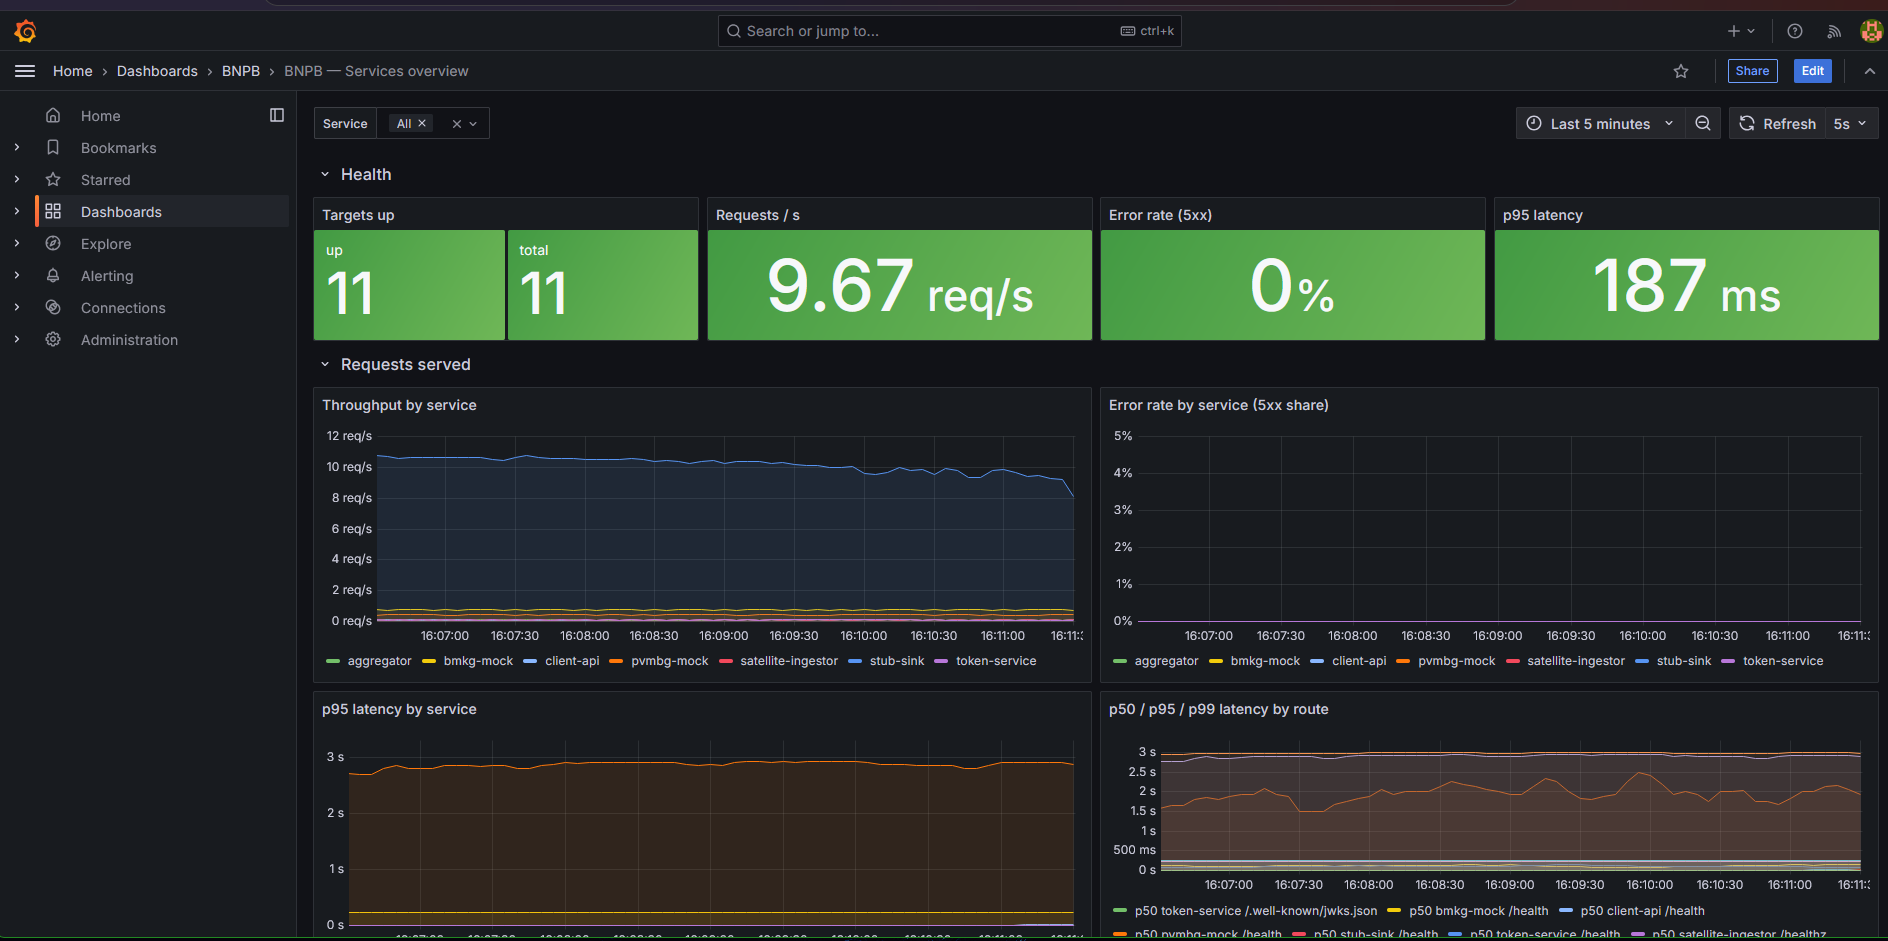
\includegraphics[width=\textwidth]{gambar/grafana-services.png}
\caption{Dashboard \textit{BNPB --- Services overview} (5 menit terakhir): 11 dari 11 target aktif, $\pm$9,7 permintaan/s, \textit{error rate} 5xx 0\%, dan p95 seluruh service 187 ms. Garis $\pm$2,9 s pada p95 per service adalah \kode{pvmbg-mock}, yang sengaja menunda setiap respons \kode{/volcanic-reports} 0,5--3 s untuk meniru sumber yang lambat.}
\end{figure}
\begin{figure}[H]\centering
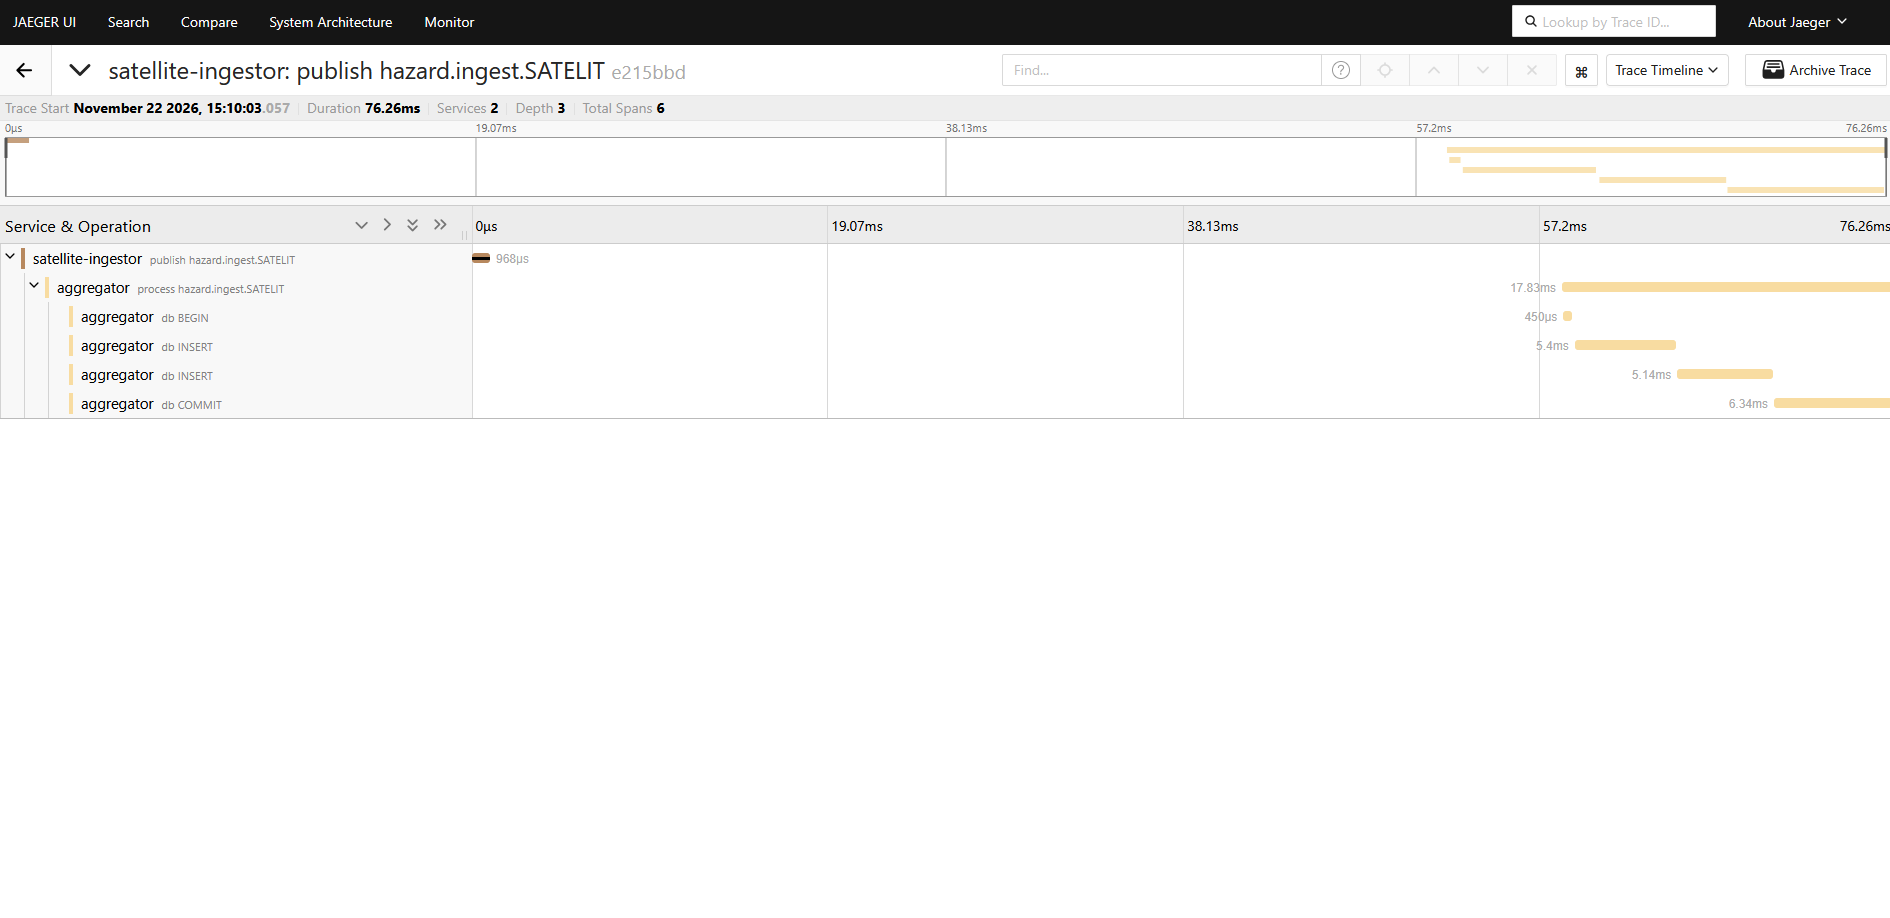
\includegraphics[width=\textwidth]{gambar/jaeger-trace.png}
\caption{Jejak satu pesan WILDFIRE lintas service di Jaeger: \kode{satellite-ingestor} mempublikasikan ke \kode{hazard.ingest.SATELIT} (0,97 ms), pesan menunggu di JetStream $\pm$57 ms, lalu Aggregator memprosesnya dalam satu transaksi CockroachDB (17,8 ms: \kode{BEGIN}, \kode{INSERT} ke \kode{canonical\_events}, \kode{INSERT} ke \textit{outbox}, \kode{COMMIT}). \textit{Trace context} diteruskan lewat header NATS.}
\end{figure}

% ─────────────────────────────────────────────────────────────
\subsection{Petunjuk Menjalankan Sistem}

Langkah lengkap ada pada \kode{README.md} bagian \textit{Kubernetes Deployment}.

\begin{enumerate}
\item \textbf{Menyiapkan klaster.} Dua VM Linux; Node A: \kode{curl -sfL https://get.k3s.io | sh -}; Node B bergabung dengan \kode{K3S\_URL} dan \kode{K3S\_TOKEN}. \kode{kubectl get nodes -o wide} menampilkan dua node \textit{Ready}.
\item \textbf{Konfigurasi.} \kode{cp .env.example .env}, isi kredensial (kunci ES256 via \kode{bash scripts/keys/gen-es256.sh}, token Feed Satelit, \kode{PANTAI\_AUTH\_TOKEN}, token audit).
\item \textbf{Deploy satu perintah:}
\begin{lstlisting}
K3S_NODES="<user>@<ip-node-a> <user>@<ip-node-b>" bash scripts/k8s/up.sh
\end{lstlisting}
Skrip membangun dan mengimpor image ke kedua node, membuat Secret, memuat dashboard Grafana, menerapkan \textit{overlay} \kode{two-node}, dan menunggu seluruh workload siap.
\item \textbf{Verifikasi platform:} \kode{bash scripts/k8s/verify.sh} (2 node berkernel terpisah, label \kode{role}, \textit{resources}, \kode{hostPath} untuk \kode{role=store}, NetworkPolicy, dan \textit{round trip} token $\rightarrow$ \kode{/v1/events}).
\item \textbf{Tester Agent:} \kode{bash scripts/k8s/tester-agent.sh install}, \kode{list}, \kode{practice <nama>}, \kode{logs}.
\item \textbf{Titik masuk:} client-api \kode{:30080}, token-service \kode{:30083}, mock \kode{:30081/:30082}, Grafana \kode{:30300}, Prometheus \kode{:30090}, Jaeger \kode{:30686}; Aggregator melalui \kode{kubectl port-forward svc/aggregator 8090:8090}.
\end{enumerate}


% ════════════════════════════ BAB II ════════════════════════════
\bab{BAB II}{Problem}
\subsection{Problem 1: Yang Pulang Membawa Laptopnya}
\tinjau{oleh Made: isi bagian ini disusun dari kode dan dokumentasi di repositori}

\subsubsection{Identifikasi Masalah}

Satu tempat penyimpanan tidak lagi cukup, dan pemecahan data ke beberapa node memunculkan beberapa persoalan:
\begin{itemize}
\item \textbf{\textit{Partitioning / sharding}}: data harus dibagi ke beberapa node agar tidak ada satu node pun yang menyimpan seluruh data atau menanggung seluruh beban tulis.
\item \textbf{\textit{Data skew / hot spot}}: gempa terkonsentrasi di jalur tertentu, sehingga partisi berdasarkan wilayah akan membuat satu node bekerja keras sementara node lain menganggur.
\item \textbf{\textit{Replication} dan \textit{fault tolerance}}: data yang hanya punya satu salinan ikut hilang bersama node-nya (``laptop dibawa pulang'').
\item \textbf{\textit{Rebalancing}}: node baru harus ikut menanggung data tanpa menghentikan baca/tulis.
\item \textbf{\textit{Scatter-gather query} dan \textit{partial results / graceful degradation}}: pembacaan lintas partisi harus menghasilkan urutan yang benar dan tetap menjawab (dengan penanda) ketika sebagian partisi tidak terjangkau.
\end{itemize}

\subsubsection{Rancangan Solusi}

\begin{enumerate}
\item \textbf{CockroachDB 4 node, \textit{RF}=3.} \kode{canonical-store} adalah StatefulSet CockroachDB v24.1.6 dengan data di disk node (\kode{hostPath}). Setiap \textit{range} direplikasi ke 3 node melalui Raft; \kode{server.time\_until\_store\_dead = 1m15s} menentukan kapan replika di node yang hilang dibuat ulang di node lain.
\item \textbf{Kunci partisi tahan \textit{skew}.} \kode{hazard\_id = "hz-" + sha256(source | source\_ref\_id)[:16]} bersifat deterministik, dan kolom terhitung \kode{shard = crc32(hazard\_id) mod 8} menjadi awalan \textit{primary key}. Tabel dan indeks di-\textit{pre-split} pada 8 nilai \textit{shard}, sehingga data dari satu wilayah yang padat tetap tersebar merata ke 8 \textit{range}.
\item \textbf{Penempatan dan perubahan node.} Penempatan replika diputuskan oleh \textit{allocator} CockroachDB berdasarkan jumlah replika dan beban per \textit{store}. Saat node baru bergabung, \textit{range} dan \textit{lease} dipindahkan otomatis ke node tersebut; saat node hilang lebih dari 1m15s, replikanya dibuat ulang dari dua salinan yang tersisa. Pada topologi 2 node, \textit{zone config} menyematkan 2 dari 3 replika ke node \textit{control plane} agar kuorum tetap ada saat node worker mati.
\item \textbf{\textit{Scatter-gather} dengan \textit{partial answer}.} Pembacaan (\kode{/internal/events}, Audit API, \kode{/internal/analytics/summary}) menjalankan query per \textit{shard} secara paralel dengan \textit{timeout} 800 ms, menggabungkan hasilnya dengan urutan \kode{(occurred\_at, hazard\_id)} dan \textit{keyset cursor}. \textit{Shard} yang gagal atau melewati batas waktu dicantumkan di \kode{unavailable\_units}, dan respons ditandai \kode{partial: true}; tidak pernah HTTP 500 atau permintaan yang menggantung.
\item \textbf{Loader katalog historis.} \kode{/loader} memuat CSV/JSON secara idempoten (\kode{ON CONFLICT DO NOTHING}); \kode{GET /internal/admin/distribution} melaporkan sebaran baris per \textit{shard} dan per node.
\item \textbf{Audit API} (\kode{/internal/audit/events}, \kode{/checksum}, \kode{/location}, \kode{/unprocessed}) dengan token audit dari Secret.
\item \textbf{Dashboard analitik} \kode{/analytics/} (Chart.js tertanam) di atas \kode{/internal/analytics/summary}: jumlah per jenis bahaya terhadap waktu, per \textit{severity}, dan per \kode{area\_name}. Gempa dengan \kode{tsunami\_warning} dihitung sebagai TSUNAMI.
\end{enumerate}

\subsubsection{Alasan Keputusan}

\begin{longtable}{|p{3cm}|p{6cm}|p{5.9cm}|}
\hline
\textbf{Alternatif} & \textbf{Konsekuensi terhadap sebaran data (kriteria 2)} & \textbf{Keputusan}\\ \hline \endhead
Partisi berdasarkan wilayah (\kode{area\_name}) & Data dan beban tulis terkonsentrasi di partisi wilayah yang padat gempa (\textit{hot spot}) & Tidak dipilih\\ \hline
Citus / PostgreSQL \textit{hash-shard} manual & Sebaran merata, tetapi replikasi, \textit{failover}, dan \textit{rebalancing} harus dioperasikan sendiri & Tidak dipilih: beban operasional tinggi\\ \hline
\textit{Consistent hashing} di aplikasi & Sebaran merata dan perpindahan data minimal saat node berubah, tetapi replikasi dan konsistensi harus dibangun sendiri & Tidak dipilih\\ \hline
CockroachDB + \textit{hash shard} (dipilih) & Hash pada \kode{hazard\_id} menyebarkan data wilayah padat secara merata; \textit{range} dipecah dan dipindahkan otomatis berdasarkan ukuran dan beban & Dipilih\\ \hline
\end{longtable}

\tinjau{oleh Made: tambahkan trade-off yang dianggap penting (misalnya biaya \textit{scatter-gather} 8 \textit{shard} untuk setiap query).}

\subsubsection{Batasan yang Disadari}
\begin{itemize}
\item Pada topologi 2 node, node \textit{control plane} menyimpan salinan setiap \textit{range}; kehilangan node \textit{control plane} tidak termasuk skenario yang ditangani.
\item Pembacaan \textit{scatter-gather} dijalankan sebagai query terpisah per \textit{shard}, sehingga hasil gabungan bukan satu \textit{snapshot} atomik lintas \textit{shard}.
\item \isi{batasan lain menurut Made}
\end{itemize}

\subsubsection{Bukti Penyelesaian}

Skrip skenario: \kode{scripts/demo/m2/p1/c1}--\kode{c7} (\kode{MODE=k8s}), bukti di \kode{evidence/p1/<run>/}.

\begin{longtable}{|p{4.2cm}|p{10.7cm}|}
\hline
\textbf{Kriteria} & \textbf{Bukti}\\ \hline \endhead
1. Dataset dimuat, tersebar & \isi{tabel sebaran per node dari \kode{c1-distribution.txt} untuk dataset asisten}\\ \hline
2. Ketidakmerataan & \isi{beban per node saat memuat dan saat lonjakan satu wilayah (\kode{c2-skew-summary.txt})}\\ \hline
3. Baca lintas lokasi & \isi{50 event terbaru + \textit{pagination} (\kode{c3-verification.txt})}\\ \hline
4. Node worker mati + data dihapus & \isi{checksum sebelum/sesudah (Audit API) dan \kode{c4-hammer.csv}: 0 HTTP 500, respons \kode{partial} selama pemulihan}\\ \hline
5. Node baru & \isi{\kode{c5-rebalance-snapshots.txt}: replika dan \textit{lease} berpindah, baca/tulis tanpa error}\\ \hline
6. Tahan kehilangan berikutnya & \isi{\kode{c6-verification.txt}}\\ \hline
7. Dashboard analitik & \isi{tangkapan layar dashboard, \kode{c7-dashboard-vs-audit.txt}, dan banner ``Data belum lengkap'' saat node mati}\\ \hline
\end{longtable}

\subsubsection{Jawaban atas Butir ``Di Laporan''}
\begin{enumerate}
\item \textbf{Persoalan dan konsep:} \textit{partitioning/sharding}, \textit{data skew / hot spot}, \textit{replication} (Raft), \textit{rebalancing}, \textit{scatter-gather} dan \textit{partial results} (lihat bagian a).
\item \textbf{Mekanisme penempatan data:} \kode{shard = crc32(hazard\_id) mod 8} menentukan \textit{range} logis; \textit{allocator} CockroachDB menentukan node yang memegang tiga replika setiap \textit{range} dan memindahkannya saat node datang (\textit{rebalancing}) atau pergi (\textit{up-replication} setelah 1m15s).
\item \textbf{Perbandingan alternatif:} lihat tabel pada bagian c.
\item \textbf{Jaminan konsistensi per endpoint:} \tinjau{oleh Made}
\begin{center}
\begin{tabularx}{\textwidth}{|p{4cm}|X|X|}
\hline
\textbf{Endpoint} & \textbf{Kondisi normal} & \textbf{Node hilang}\\ \hline
\kode{GET /v1/events}, \kode{/internal/events} & Setiap \textit{shard} dibaca konsisten dari \textit{leaseholder} (\textit{serializable}); hasil gabungan terurut, tetapi bukan satu \textit{snapshot} atomik lintas \textit{shard} & \textit{Shard} yang \textit{range}-nya sedang berpindah \textit{lease} dapat melewati batas 800 ms: data yang ada dikembalikan dengan \kode{partial: true} dan \kode{unavailable\_units} (ketersediaan diutamakan)\\ \hline
Audit API \kode{events}/\kode{checksum} & Sama, dengan urutan \kode{(ingested\_at, hazard\_id)} & Sama; \textit{checksum} parsial ditandai sehingga tidak disalahartikan sebagai lengkap\\ \hline
\kode{/internal/analytics/summary} & Agregasi per \textit{shard} lalu dijumlahkan & Angka ditampilkan dengan awalan $\ge$ dan banner ``belum lengkap''\\ \hline
Penulisan (\textit{upsert}) & Transaksi \textit{serializable} dengan kuorum Raft & Tetap berhasil selama kuorum setiap \textit{range} terpenuhi\\ \hline
\end{tabularx}
\end{center}
\item \textbf{Agregasi dashboard lintas lokasi:} setiap \textit{shard} menghitung agregat sendiri secara paralel, lalu Aggregator menjumlahkannya. \textit{Shard} yang tidak menjawab dalam 800 ms tidak dihitung, dicantumkan di \kode{unavailable\_units}, dan dashboard menampilkan banner serta awalan $\ge$ pada angka. Kesamaan dengan Audit API diverifikasi oleh \kode{scripts/p1/dashboard-vs-audit.sh}.
\end{enumerate}

\subsection{Problem 2: Dua Nakhoda, Satu Kapal}

\subsubsection{Identifikasi Masalah}
\begin{itemize}
\item \textbf{Kriteria 2 --- \textit{Leader election / mutual exclusion} dan \textit{effectively-once ingestion}:} tiga instance yang sama-sama melakukan \textit{polling} menggandakan permintaan ke upstream dan event di penyimpanan. Dibutuhkan tepat satu pemimpin aktif yang melakukan \textit{polling}, disertai penulisan idempoten agar pergantian pemimpin tidak menimbulkan duplikat maupun celah data.
\item \textbf{Kriteria 4 --- \textit{Unreliable clocks / clock skew} dan \textit{split-brain}:} jam fisik (\textit{wall-clock}) antar mesin bisa bergeser maju maupun mundur (+45 s / $-$30 s). Jika keabsahan \textit{lease} dihitung memakai jam lokal node Aggregator, dua instance bisa sama-sama merasa menjadi \textit{leader} (\textit{split-brain}) dan menulis bersamaan.
\item \textbf{Kriteria 5 --- \textit{Process pause / zombie leader} dan \textit{fencing token}:} \textit{leader} yang membeku (\textit{suspend} VM atau jeda GC panjang) melebihi batas waktu \textit{lease} tidak tahu bahwa kepemimpinannya sudah pindah ke instance lain. Ketika bangun kembali (\textit{zombie leader}), ia dapat menulis data basi ke penyimpanan. Penanganannya adalah \textit{fencing token} yang naik monoton dan diperiksa di sisi penyimpanan (Kleppmann, 2016. 2017, bab 8).
\item \textbf{Kriteria 6--8:} \textit{horizontal scaling} di bawah beban, \textit{load balancing} berbasis \textit{readiness}, dan \textit{rolling update} tanpa \textit{downtime}.
\end{itemize}

\subsubsection{Rancangan Solusi}
\begin{enumerate}
\item \textbf{Titik masuk tunggal dan \textit{graceful drain}.} Deployment \kode{aggregator} berjalan dengan 3 replika (\textit{soft podAntiAffinity} dan \kode{topologySpreadConstraints} per host) di belakang Service \kode{aggregator:8090}. Saat menerima \kode{SIGTERM}, \kode{GET /internal/ready} segera mengembalikan \kode{503 DRAINING}, worker dihentikan, \textit{lease} dilepas secara sukarela, dan pod menunggu \kode{preStop} / \kode{SHUTDOWN\_DRAIN\_S} 5 s agar \kode{kube-proxy} memutus trafik baru sebelum server HTTP ditutup. Strategi \textit{rolling update} memakai \kode{maxUnavailable: 0}, \kode{maxSurge: 1}.
\item \textbf{\textit{Lease} di CockroachDB (sumber kebenaran waktu = HLC \kode{now()}).} Tabel \kode{leader\_leases} diperbarui lewat \kode{AcquireOrRenewLease}. Seluruh perhitungan dan perbandingan kedaluwarsa (\kode{expires\_at > now()}) memakai \kode{now()} milik CockroachDB yang dijaga \textit{Hybrid Logical Clock} (HLC), tidak pernah memakai jam OS node Aggregator. Perpanjangan oleh pemegang sah mempertahankan \kode{fencing\_token}. Pengambilalihan setelah kedaluwarsa selalu menaikkan \kode{fencing\_token + 1}.
\item \textbf{\textit{Renew-before-poll}.} Sebelum mengirim permintaan ke BMKG/PVMBG pada setiap siklus, pemimpin memanggil \kode{elector.RenewNow()} secara sinkron ke DB. Jika \textit{zombie leader} baru bangun dari \textit{freeze}, panggilan ini langsung gagal dan instance mendemosi dirinya (\kode{leader\_lost}) tanpa menyentuh upstream.
\item \textbf{\textit{Fencing token} pada transaksi tulis (\kode{UpsertFencedBatch}).} Jika pemimpin membeku \textit{setelah} membaca upstream namun \textit{sebelum} menulis ke DB, \kode{UpsertFencedBatch} memverifikasi \kode{holder}, \kode{fencing\_token}, dan \kode{expires\_at > now()} di dalam transaksi \textit{serializable} yang sama dengan \textit{upsert} event, \textit{outbox}, dan pemajuan \textit{watermark}. Bila token sudah usang, transaksi di-\textit{rollback} (\kode{ErrFenced}, 0 baris tertulis) dan instance mendemosi dirinya.
\item \textbf{\textit{Watermark} durable dan idempotensi.} Tabel \kode{poller\_watermarks} menyimpan posisi terakhir secara atomik bersama batch tulis. Pemimpin baru memuat \textit{watermark} ini dengan mundur aman \kode{watermarkOverlap = 1 s} agar tidak ada event yang terlewat di batas detik, sementara kunci deterministik \kode{hazard\_id} (\kode{ON CONFLICT DO NOTHING/UPDATE}) mencegah duplikat. Mock mencatat permintaan per instance pada \kode{/admin/requests} untuk pembuktian.
\item \textbf{Uji beban (Fayadh).} k6 dijalankan dari luar klaster dengan skrip \kode{scripts/demo/m2/load/} (konfigurasi pada butir ``Di Laporan'' 4).
\end{enumerate}

\subsubsection{Alasan Keputusan}
\begin{itemize}
\item \textbf{\textit{Lease} di CockroachDB vs.\ Kubernetes \kode{Lease}:} \textit{fencing} hanya aman jika diperiksa tepat di tempat penulisan terjadi. Dengan menaruh \kode{leader\_leases} di CockroachDB yang sama, pengecekan \kode{fencing\_token} dan penulisan data berjalan atomik dalam satu transaksi \textit{serializable}, serta memakai satu sumber waktu (HLC CockroachDB). Kubernetes \kode{Lease} tidak bisa memagari transaksi SQL di basis data dan rentan terhadap pergeseran jam klien.
\item \textbf{Penetapan batas waktu dan \textit{trade-off}:} \kode{config.Load()} memvalidasi secara ketat bahwa \kode{LEASE\_TTL\_S > 2 * LEASE\_RENEW\_INTERVAL\_S}.
\begin{center}
\begin{tabularx}{\linewidth}{|p{4.3cm}|p{1.3cm}|X|}
\hline
\textbf{Parameter} & \textbf{Nilai} & \textbf{Fungsi dan \textit{trade-off}}\\ \hline
\kode{LEASE\_TTL\_S} & 15 s & Masa berlaku \textit{lease}. \textit{Worst-case failover} $\approx$ 15 + 5 = 20 s (jauh di bawah batas 60 s). Nilai terlalu kecil (mis.\ 5 s) memicu \textit{false failover} saat jeda GC/jaringan singkat. Nilai terlalu besar (mis.\ 45 s) mendesak \textit{failover} ke batas 60 s.\\ \hline
\kode{LEASE\_RENEW\_INTERVAL\_S} & 5 s & Jeda perpanjangan \textit{lease}. Memberi 3 kali kesempatan perpanjangan dalam 15 s sehingga gangguan satu permintaan tidak menjatuhkan \textit{leader}, sambil menjaga beban tulis sangat rendah (0,2 \textit{writes}/s).\\ \hline
\kode{safetyMargin} lokal & 2 s & Pemimpin lokal berhenti menganggap dirinya aktif pada 13 s tanpa perpanjangan sukses, sebagai rem konservatif sebelum \textit{lease} benar-benar habis di DB.\\ \hline
\kode{SHUTDOWN\_DRAIN\_S} & 5 s & Waktu tunggu setelah \kode{/internal/ready} mengembalikan 503 agar \textit{load balancer} menghentikan trafik baru sebelum proses keluar, tanpa melewati batas terminasi pod 30 s.\\ \hline
\kode{watermarkOverlap} & 1 s & Mundur 1 s saat \textit{polling} untuk mencegah celah di batas detik. Memicu pembacaan ulang beberapa event terbaru namun aman karena \textit{upsert} idempoten.\\ \hline
\end{tabularx}
\end{center}
\item \textbf{Uji beban dengan satu token per client:} 10.000 VU yang masing-masing meminta token akan menguji token-service, bukan jalur baca. Karena itu TTL token dinaikkan selama uji dan \textit{rate limit} per client dibuka (semua VU memakai satu client).
\end{itemize}

\subsubsection{Batasan yang Disadari}
\begin{itemize}
\item Keselamatan waktu bergantung pada batas \kode{--max-offset = 500 ms} CockroachDB. Jika jam OS pada sebuah node store melampaui 500 ms, node store tersebut mematikan dirinya sendiri untuk menjaga konsistensi HLC (mengurangi sementara kapasitas store).
\item Jika pemimpin membeku \textit{setelah} mengirim HTTP GET ke upstream tetapi \textit{sebelum} menulis ke DB, satu panggilan baca upstream tidak dapat dibatalkan. Namun \kode{UpsertFencedBatch} menjamin 0 baris basi ditulis ke basis data.
\item Uji beban 10.000 VU dari satu mesin dibatasi CPU, \textit{port}, dan jaringan mesin penguji. \isi{batasan yang teramati di klaster demo}
\end{itemize}

\subsubsection{Bukti Penyelesaian}

Skrip: \kode{scripts/demo/m2/p2/c1}--\kode{c5} (\kode{MODE=k8s}) dan \kode{scripts/demo/m2/load/}.

\begin{longtable}{|p{4.2cm}|p{10.7cm}|}
\hline
\textbf{Kriteria} & \textbf{Bukti}\\ \hline \endhead
1. 3 instance, satu titik masuk & \isi{\kode{c1-verification.txt}: instance yang di-\textit{drain} keluar dari \textit{endpoints}, 100\% HTTP 200}\\ \hline
2. Tepat sekali & \isi{\kode{c2}: \kode{duplicates: []} pada log mock, 0 duplikat \kode{(source, source\_ref\_id)}}\\ \hline
3. \textit{Failover} $\le$ 60 s & \isi{\kode{c3}: waktu pengambilalihan, \kode{fencing\_token} naik, 0 celah/duplikat (\kode{KILL\_MODE=node})}\\ \hline
4. \textit{Clock skew} +45/$-$30 s & \isi{\kode{c4-write-intervals.txt}: interval penulisan per \textit{epoch} tidak beririsan}\\ \hline
5. \textit{Freeze} & \isi{\kode{c5}: instance yang bangun tidak menulis (\kode{write rejected: stale fencing token})}\\ \hline
6. 10.000 VU, 3, 5, lalu 2 & \isi{\kode{evidence/load/<run>/verdict.txt}: total request, error tak terduga (\%), p95, error per fase. \kode{replicas.csv}}\\ \hline
7. \textit{Throughput} 3 vs 1 & \isi{\kode{throughput.sh}: served/s 1 replika, 3 replika, rasio}\\ \hline
8. \textit{Rolling update} & \isi{error fase \kode{rolling\_update} = 0}\\ \hline
\end{longtable}

\subsubsection{Jawaban atas Butir ``Di Laporan''}
\begin{enumerate}
\item \textbf{Persoalan:} kriteria 2 \textit{leader election / mutual exclusion} dan \textit{effectively-once ingestion}. Kriteria 4 \textit{unreliable clocks / clock skew} yang memicu \textit{split-brain}. Kriteria 5 \textit{process pause / zombie leader} yang dicegah dengan \textit{fencing token}.
\item \textbf{Mekanisme dan sumber waktu:} \textit{lease} di CockroachDB dengan \kode{now()} HLC sebagai satu-satunya otoritas waktu, dilengkapi \textit{renew-before-poll} dan pemeriksaan \kode{fencing\_token} di dalam transaksi \textit{serializable} penulisan. Pergeseran jam +45 s / $-$30 s pada node Aggregator (kriteria 4) tidak memengaruhi keputusan \textit{lease} karena jam lokal tidak pernah dibandingkan di DB. Instance yang bangun dari \textit{freeze} (kriteria 5) gagal pada \textit{renew-before-poll} atau ditolak oleh \kode{UpsertFencedBatch} (\kode{ErrFenced}) karena membawa \textit{token} lama, sehingga 0 baris basi tertulis.
\item \textbf{Batas waktu:} \textit{lease TTL} 15 s, perpanjangan 5 s, margin keselamatan lokal 2 s, \textit{shutdown drain} 5 s, dan \textit{watermark overlap} 1 s. \textit{worst-case failover} $\approx$ 20 s. Analisis \textit{trade-off} tiap nilai disajikan pada tabel bagian Alasan Keputusan di atas.
\item \textbf{Konfigurasi uji beban:}
\begin{center}
\begin{tabularx}{\textwidth}{|p{3.6cm}|X|}
\hline
Alat dan lokasi & k6 \isi{versi} di \isi{mesin di luar klaster}, menembak NodePort client-api (\kode{tests/load/k6\_m2.js})\\ \hline
Beban & 10.000 VU, \textit{ramp} 30 s, ditahan 150 s, jeda 0,5 s per iterasi, \kode{GET /v1/events?limit=20} dengan token Tim Lapangan\\ \hline
Jadwal & 0 s: 3 replika. 20 s: 5. 60 s: 2. 95 s: \textit{rolling update} (image baru atau revisi \textit{pod template})\\ \hline
Pengaturan selama uji & \textit{Rate limit} per client dibuka, TTL token 900 s (satu token per client dari \kode{setup()}), \textit{trace sampling} 1\%. Seluruhnya dikembalikan setelah uji\\ \hline
Klasifikasi & 200 dilayani. 429/503 penolakan terkontrol. Selain itu error. \textit{Threshold}: error $<$ 1\% dan 0 error pada fase \kode{rolling\_update}\\ \hline
\textit{Throughput} & 600 VU, 60 s per konfigurasi (1 lalu 3 replika), client-api 4 replika\\ \hline
\end{tabularx}
\end{center}
\end{enumerate}

\subsection{Problem 3: Surat dari Tetangga}
\tinjau{oleh Theo untuk kriteria 1--5; kriteria 6 oleh Fayadh}

\subsubsection{Identifikasi Masalah}
\begin{itemize}
\item \textbf{Kriteria 2: \textit{schema evolution} yang tidak kompatibel dan \textit{dead-letter queue}.} Pesan yang tidak dapat diproses harus disimpan utuh beserta alasannya, dan kegagalan sementara (\textit{transient}) harus dibedakan dari kegagalan permanen (\textit{non-retryable}). Konsep: \textit{Dead Letter Channel} (Hohpe \& Woolf), \textit{retry with backoff}.
\item \textbf{Kriteria 3: \textit{poison message}.} Pesan rusak (JSON terpotong, bersarang sangat dalam, UTF-8 tidak valid, ukuran berlebih) tidak boleh membuat komponen \textit{crash} atau terus \textit{restart}. Konsep: validasi input, batas sumber daya, isolasi kegagalan per pesan.
\item \textbf{Kriteria 4: \textit{idempotent replay} dengan urutan per kunci.} Pemrosesan ulang tidak boleh menghasilkan duplikat dan harus mempertahankan urutan per \kode{source\_ref\_id}.
\item \textbf{Kriteria 6: \textit{guaranteed delivery} / \textit{store-and-forward}.} Laporan Tim Lapangan yang dibalas 202 tidak boleh hilang walaupun penerima mati setelah membalas, dan tidak boleh diproses ganda. Konsep: \textit{acknowledgement} setelah persistensi, \textit{at-least-once delivery}, \textit{idempotent receiver}, \textit{effectively-once processing}.
\end{itemize}

\subsubsection{Rancangan Solusi}

\textbf{Perubahan skema PVMBG (Theo).} Mock PVMBG mendapat mode \kode{POST /admin/schema-version?mode=incompatible} (\kode{volcano\_id} $\rightarrow$ \kode{volcano\_code}, \kode{ash\_column\_height\_m} menjadi string, \kode{reported\_at} dihapus). Aggregator memvalidasi setiap laporan sebelum normalisasi:

\begin{center}
\begin{tabularx}{\textwidth}{|X|X|}
\hline
\textbf{Perubahan} & \textbf{Perlakuan}\\ \hline
Field baru & Diterima, disimpan di \kode{attributes}\\ \hline
Field opsional hilang & Diterima\\ \hline
Field wajib hilang, \textit{rename}, perubahan tipe & Ditolak: \textbf{parked} di DLQ\\ \hline
JSON terpotong, UTF-8 tidak valid, body $>$ 1 MiB, \textit{nesting} $>$ 32 & Ditolak: \textbf{parked}\\ \hline
Basis data atau kegagalan sementara lain & \textbf{retrying} dengan \textit{backoff} 5 s $\rightarrow$ 10 menit, \textit{parked} setelah 5 percobaan\\ \hline
\textit{Panic} saat memproses satu pesan & Dipulihkan, pesan di-\textit{park}, service tetap berjalan\\ \hline
\end{tabularx}
\end{center}

DLQ adalah tabel \kode{dead\_letters} yang menyimpan pesan mentah \textit{byte} demi \textit{byte} beserta \kode{reason}, \kode{source}, \kode{received\_at}, \kode{retryable}, \kode{attempts}, dan \kode{status} (\kode{retrying}/\kode{parked}/\kode{resolved}). \textit{Watermark polling} hanya maju setelah setiap pesan tersimpan atau aman di DLQ. \textit{Replay} (\kode{POST /internal/dlq/replay}) memproses ulang pesan \textit{parked} dengan normalizer terbaru; hasilnya di-\textit{upsert} berdasarkan \kode{(source, source\_ref\_id)} dan urutan per \kode{source\_ref\_id} dipertahankan. Pemeriksaan DLQ hanya untuk BNPB Internal Ops (\kode{INTERNAL\_OPS\_TOKEN}) dan Audit API (\kode{/internal/audit/unprocessed}). Ingest dari sumber lain (\kode{hazard.ingest.*}) memakai DLQ yang sama untuk pesan rusak dan data yang ditolak sumbernya (\kode{op=reject}, lihat P5).

\textbf{Laporan Tim Lapangan (Fayadh).}
\begin{enumerate}
\item \kode{POST /field-reports}: \textit{scope} \kode{field\_team}/\kode{internal\_ops} (Media 403), body $\le$ 64 KB, JSON ketat, field wajib, \kode{Idempotency-Key} (atau \kode{report\_id}) wajib.
\item Laporan dipublikasikan ke stream \kode{FIELD\_REPORTS} (\textit{file storage}) dengan \kode{Nats-Msg-Id = <client\_id>/<key>}. \textbf{Balasan 202 baru dikirim setelah PubAck}; tanpa \textit{ack} dalam 2 s, balasan 503 + \kode{Retry-After} (tidak pernah 202 palsu).
\item Pengiriman ulang dengan \textit{key} yang sama dibuang JetStream (\textit{duplicate window} 2 jam); client tetap menerima 202 dengan \kode{"duplicate": true}.
\item \kode{field-report-consumer}: \textit{durable pull consumer}, \textit{redelivery} tanpa batas dengan \textit{backoff} 1--30 s; mengirim ke penerima dengan \kode{Idempotency-Key}, mencatat ID di bbolt, \textbf{baru kemudian} \textit{ack}.
\item Penerima (\kode{stub-sink}) menyimpan setiap \textit{message ID} sekali (menutup celah \textit{crash} antara jawaban penerima dan penulisan bbolt).
\end{enumerate}

\subsubsection{Alasan Keputusan}
\begin{itemize}
\item \textbf{DLQ di tabel basis data vs stream terpisah:} \tinjau{oleh Theo}
\item \textbf{Menolak perubahan tidak kompatibel vs menebak isinya:} menebak pemetaan (misalnya \kode{volcano\_code} dianggap \kode{volcano\_id}) berisiko menyimpan data salah tanpa jejak; menyimpan utuh dan memproses ulang setelah normalizer diperbarui menjaga kebenaran data. \tinjau{oleh Theo}
\item \textbf{202 setelah PubAck vs menulis langsung ke basis data:} menulis ke basis data dari client-api melanggar kepemilikan storage dan membuat latensi bergantung pada basis data; balasan 202 sebelum publish berisiko kehilangan laporan bila client-api mati.
\item \textbf{Dedup di setiap hop vs \textit{exactly-once} broker saja:} efek samping di penerima tetap memerlukan dedup; kombinasi \textit{at-least-once} + dedup lebih sederhana dan terbukti.
\end{itemize}

\subsubsection{Batasan yang Disadari}
\begin{itemize}
\item NATS berjalan satu instance (R1): bila node \textit{control plane} mati total, jalur tulis laporan berhenti (client menerima 503, tidak pernah 202 palsu). JetStream melakukan \textit{fsync} secara berkala, sehingga kehilangan daya mendadak pada node broker masih menyisakan risiko kecil; \textit{crash} proses dan \textit{pod} aman.
\item \isi{batasan DLQ/replay menurut Theo}
\end{itemize}

\subsubsection{Bukti Penyelesaian}

\begin{longtable}{|p{4.2cm}|p{10.7cm}|}
\hline
\textbf{Kriteria} & \textbf{Bukti}\\ \hline \endhead
1. Deklarasi kebijakan & Tabel kebijakan di atas; \isi{tangkapan layar perilaku pada mock PVMBG mode \kode{incompatible}}\\ \hline
2. Pesan tersimpan, \textit{retrying} vs \textit{parked} & \isi{query \kode{dead\_letters} / \kode{GET /internal/dlq?status=parked}}\\ \hline
3. Pesan rusak & \isi{\kode{go test ./internal/schema/ ./internal/dlq/ ./internal/poller/} dan \kode{kubectl get pods} (0 \textit{restart})}\\ \hline
4. \textit{Replay} & \isi{hasil \kode{/internal/dlq/replay}: \kode{resolved}, 0 duplikat, urutan per \kode{source\_ref\_id}}\\ \hline
5. Hanya Internal Ops & \isi{401 tanpa token / token salah, 200 dengan token Internal Ops}\\ \hline
6. Laporan Tim Lapangan & Klaster pengembangan (\kode{scripts/demo/m2/field-reports/field-reports.sh}, N=150): consumer dimatikan $\rightarrow$ 20/20 dibalas 202 (p95 20 ms); client-api dan consumer di-SIGKILL di tengah pengiriman $\rightarrow$ 170 dibalas 202, 170 sampai di penerima, 0 hilang, 0 diproses ganda, 150/150 pengiriman ulang dijawab \kode{duplicate: true}; broker mati $\rightarrow$ 503 dalam 8 ms. Klaster demo: \isi{hasil N=200 dari \kode{evidence/field-reports/<run>/}}\\ \hline
\end{longtable}

\subsubsection{Jawaban atas Butir ``Di Laporan''}
\begin{enumerate}
\item \textbf{Persoalan:} kriteria 2 \textit{dead letter channel} dan pembedaan \textit{retryable/non-retryable}; kriteria 3 \textit{poison message}; kriteria 4 \textit{idempotent replay} dengan \textit{per-key ordering}; kriteria 6 \textit{guaranteed delivery} dengan \textit{idempotent receiver}.
\item \textbf{Kebijakan skema:} perubahan aditif dan field opsional yang hilang diterima otomatis; \textit{rename}, perubahan tipe, field wajib hilang, dan pesan rusak ditolak ke DLQ. \tinjau{oleh Theo: alasan pemilihan}
\item \textbf{Penyimpanan, pemeriksaan, pemrosesan ulang:} tabel \kode{dead\_letters}; diperiksa lewat \kode{/internal/dlq} (Internal Ops) dan \kode{/internal/audit/unprocessed}; \textit{replay} melalui normalizer terbaru dengan \textit{upsert} \kode{(source, source\_ref\_id)} sehingga tidak ada duplikat.
\item \textbf{Jaminan pengiriman laporan Tim Lapangan:} \textit{at-least-once} dari JetStream + dedup \textit{message ID} di setiap hop (\textit{duplicate window} JetStream, bbolt di consumer, penerima idempoten) = setiap laporan yang dibalas 202 diproses tepat sekali secara efektif. Bukti: baris kriteria 6 pada tabel di atas.
\end{enumerate}

\subsection{Problem 4: Atap Seng di Siang Bolong}

\subsubsection{Identifikasi Masalah}
\begin{itemize}
\item \textbf{Kriteria 2: \textit{event time vs processing time}, \textit{watermark} dan \textit{allowed lateness}.} Deteksi harus dikelompokkan berdasarkan waktu lintasan satelit, bukan waktu tiba. Data yang terlambat harus diberi batas yang dinyatakan dan dihitung bila melewatinya (Akidau dkk., \textit{The Dataflow Model}, dan \textit{Streaming Systems}).
\item \textbf{Kriteria 4: \textit{backpressure} dan \textit{consumer lag}} saat aliran dipercepat 60$\times$. Latensi dari masuk sampai tersimpan harus terukur.
\item \textbf{Kriteria 5: \textit{stateful stream processing} dengan \textit{checkpoint} dan \textit{exactly-once processing}.} Keadaan kebakaran yang sedang dibentuk dan posisi baca harus tersimpan secara atomik agar \textit{crash} tidak menghilangkan atau menggandakan kebakaran.
\item \textbf{Kriteria 1 dan 3:} pengelompokan berantai (\textit{connected components}) dan \textit{stable identifiers} untuk kebakaran yang diperbarui, digabung, atau ditarik.
\end{itemize}

\subsubsection{Rancangan Solusi}

\begin{longtable}{|p{3.5cm}|p{11.4cm}|}
\hline
\textbf{Aspek} & \textbf{Desain}\\ \hline \endhead
Pengambilan data & \kode{GET /v1/stream} (SSE, token grup dari Secret). \textit{Reconnect} dengan \kode{?from=<offset>}. 400/401 menghentikan service. 429/503 \textit{backoff} eksponensial (menghormati \kode{Retry-After}). 45 s tanpa \textit{byte} memicu \textit{reconnect}.\\ \hline
Lanjut setelah \textit{restart} & \textit{Offset} berikutnya disimpan di PostgreSQL \textbf{dalam transaksi yang sama} dengan perubahan kebakaran.\\ \hline
Definisi kebakaran & Dedup \kode{satellite|acq\_date|acq\_time|lat|lon}. Buang \textit{confidence} rendah. Hubungkan deteksi $\le$ 1 km dan $\le$ 360 menit secara berantai. $\ge$ 2 deteksi = kebakaran. Deteksi tunggal dihitung.\\ \hline
Waktu & Seluruh logika memakai waktu akuisisi deteksi (UTC), bukan waktu tiba.\\ \hline
Keterlambatan & Deteksi yang lebih tua 2 jam dari deteksi terbaru yang pernah dilihat dihitung sebagai \textit{late} dan tidak dikelompokkan (\kode{satellite\_durable\_count\{kind="late"\}}).\\ \hline
\textit{Update}/\textit{retract} & Mengubah deteksi tersimpan dan mengelompokkan ulang hanya kebakaran terkait. Deteksi yang ditarik tetap disimpan dengan tanda.\\ \hline
ID stabil & \kode{source\_ref\_id} diawali hash kunci deteksi paling awal, lalu dibawa ke kebakaran hasil hitung ulang yang beririsan. Saat digabung, kebakaran lama mempertahankan ID dan yang lain dikirim sebagai \textit{delete}.\\ \hline
Pemetaan & WILDFIRE/SATELIT. Lokasi berupa \textit{centroid}. \kode{occurred\_at} deteksi paling awal. Provinsi terdekat (tabel statis 38 provinsi). \textit{Severity} AWAS ($\ge$ 20 deteksi atau $\ge$ 100 MW), SIAGA ($\ge$ 6 atau $\ge$ 30 MW), WASPADA. \kode{attributes}: \kode{detection\_count}, \kode{satellites}, \kode{max\_confidence}, \kode{total\_frp\_mw}, \kode{detection\_keys}.\\ \hline
Pengiriman ke Aggregator & \textit{Outbox} dalam transaksi yang sama, dipublikasikan ke \kode{hazard.ingest.SATELIT} dengan \kode{Nats-Msg-Id}. \kode{source\_version} = \textit{offset} feed sehingga keadaan terbaru selalu menang. Bila satu kebakaran punya beberapa baris \textit{outbox} yang belum terkirim, \textit{relay} hanya mengirim yang terbaru dan menandai yang lama sebagai tergantikan (\kode{satellite\_outbox\_superseded\_total}), karena Aggregator tetap hanya menyimpan versi tertinggi. Ini mencegah lonjakan \textit{update} saat mengejar \textit{backlog} membanjiri Aggregator.\\ \hline
Duplikat dari feed & Feed mengirim ulang sebagian deteksi. Kunci yang sudah pernah disimpan diabaikan dan dihitung sebagai \textit{duplicate}, sehingga salinan ulang tidak membatalkan \textit{update} yang datang kemudian dan tidak menghidupkan kembali deteksi yang sudah ditarik.\\ \hline
Pengelompokan ulang & Hanya bagian yang terdampak satu pesan: tetangga langsung deteksi baru ($\le$ 1 km, $\le$ 360 menit) beserta kebakaran tempat tetangga itu berada, atau kebakaran yang memuat deteksi yang diubah. Kebakaran tersimpan adalah komponen terhubung yang lengkap, sehingga tidak ada deteksi lain yang dapat ikut terhubung. Hasilnya sama dengan mengelompokkan ulang seluruh data, tanpa biaya yang tumbuh dengan jumlah data.\\ \hline
Event rusak & Baris lebih dari 1 MiB, JSON rusak, deteksi tidak valid, dan \textit{panic} saat memproses satu pesan disimpan di \kode{satellite\_dead\_letters} beserta \textit{byte} mentahnya. \textit{Offset} tetap maju sehingga satu event rusak tidak menghentikan aliran.\\ \hline
\end{longtable}

\subsubsection{Alasan Keputusan}
\begin{itemize}
\item \textbf{SSE + \textit{offset} vs \textit{polling} M1:} Aliran berbasis \textit{offset} monoton memberi posisi baca yang tepat untuk dilanjutkan, tanpa \textit{watermark} waktu yang bisa melewatkan atau mengulang data seperti pada \textit{polling} berbasis \kode{since}.
\item \textbf{Keadaan di PostgreSQL milik ingestor vs JetStream KV:} \textit{offset}, deteksi, kebakaran, dan \textit{outbox} perlu diperbarui atomik. Satu transaksi PostgreSQL memberikannya tanpa protokol dua fase. JetStream KV tidak dapat ikut dalam transaksi yang sama dengan tabel kebakaran, sehingga \textit{crash} di antara dua penulisan dapat membuat \textit{offset} dan keadaan tidak sinkron.
\item \textbf{Batas keterlambatan 2 jam:} batas yang lebih besar menerima lebih banyak deteksi terlambat, tetapi kebakaran baru stabil lebih lama dan lebih banyak keadaan lama yang harus dihitung ulang. Batas yang lebih kecil membuang lebih banyak data. Dua jam jauh lebih pendek dari jendela penghubung 360 menit, sehingga deteksi yang diterima masih dapat menyambung ke kebakaran yang sedang dibentuk. Pada feed latihan (181.467 event), batas ini menghitung 4.845 deteksi (2,7\%) sebagai \textit{late}. Sisanya diterima. Nilainya diukur dari waktu deteksi terbaru yang pernah dilihat (\textit{watermark} \textit{event time}), bukan dari jam dinding, karena feed berjalan pada waktu virtual 60$\times$.
\end{itemize}

\subsubsection{Batasan yang Disadari}
\begin{itemize}
\item \kode{satellite-ingestor} berjalan satu replika (\textit{Recreate}). Dua replika bersamaan akan membaca feed dua kali.
\item Pemetaan provinsi memakai jarak ke ibu kota provinsi, sehingga titik dekat perbatasan dapat dinamai provinsi tetangga.
\item Deteksi yang melewati batas keterlambatan hanya dihitung, tidak disimpan, sehingga tidak dapat dikelompokkan belakangan bila batas diubah.
\item Event satelit yang rusak tersimpan di \kode{satellite\_dead\_letters}, terpisah dari DLQ Aggregator, sehingga tidak muncul di \kode{/internal/audit/unprocessed}.
\item Uji \textit{kill-and-restart} memakai rekaman feed profil \textit{practice}. Profil ujian asisten tidak diuji.
\item Jaeger menyimpan 5\% \textit{trace} \kode{satellite-ingestor}, sehingga tidak setiap pesan dapat dilacak.
\item Pada Docker Compose, satu Aggregator menerapkan $\pm$10--20 pesan/s karena setiap pesan, termasuk versi lama yang diabaikan, memerlukan satu transaksi CockroachDB. Sebelum \textit{relay} menggabungkan versi per kebakaran, ingestor yang sedang mengejar \textit{backlog} mengirim lebih cepat dari itu dan antrean Aggregator sempat mencapai $\pm$158 ribu pesan. Latensi p50/p95/p99 pada kriteria 4 diukur di ingestor (dari baca sampai komit), bukan sampai HazardEvent tersimpan di \kode{canonical\_events}.
\end{itemize}

\subsubsection{Bukti Penyelesaian}

\begin{longtable}{|p{4.2cm}|p{10.7cm}|}
\hline
\textbf{Kriteria} & \textbf{Bukti}\\ \hline \endhead
\multicolumn{2}{|p{14.9cm}|}{Bukti kriteria 1--4, 7, dan 8 dikumpulkan oleh \kode{scripts/demo/m2/p4/p4.sh} ke \kode{evidence/p4/<run>/}. Angka di bawah diambil dari \kode{summary.txt} run \kode{20261122T073253Z} (Docker Compose) kecuali disebut lain.}\\ \hline
1. WILDFIRE & \kode{satellite-fires-top.txt} dan \kode{canonical-wildfire-top.txt}: contoh HazardEvent WILDFIRE \kode{1d7fd1e3\ldots}, AWAS, Jawa Timur, \kode{occurred\_at} 2026-12-03 03:34 UTC, 62 deteksi. Setelah antrean Aggregator habis, \kode{satellite-store} berisi 7.980 kebakaran dan \kode{canonical\_events} berisi 7.920 WILDFIRE aktif serta 18 yang dihapus. Selisih 60 adalah pesan yang masih dalam perjalanan. Sebaran \textit{severity} di \kode{satellite-store}: 7.557 AWAS, 29 WASPADA, karena total FRP dijumlahkan sepanjang umur kebakaran.\\ \hline
2. Waktu deteksi, keterlambatan & Pada feed latihan: 4.845 \textit{late}, 19.883 \textit{confidence} rendah, 9.259 duplikat dari 181.467 event. Feed \textit{live} (483.254 \textit{offset}): 13.033 \textit{late}, 53.075 \textit{confidence} rendah, 24.602 duplikat, 5.474 kunci tak dikenal, 0 tidak valid, 0 \textit{dead letter}.\\ \hline
3. \textit{Update}/\textit{retract} & \kode{stable-id-history.txt}: kebakaran \kode{fb89a3a5\ldots} mempertahankan \kode{source\_ref\_id} yang sama selama 101 versi. 30 pesan \textit{delete} (kebakaran yang tergabung atau kosong) dan 8.129 deteksi ditarik. Kasus penarikan deteksi paling awal, penggabungan, dan pemisahan diuji di \kode{internal/ingest}.\\ \hline
4. 60$\times$, p95 latensi & Pada rekaman feed latihan (uji \kode{internal/e2e}, tanpa jaringan), pemrosesan $\pm$385 event/s. Feed \textit{live} 60$\times$ (Compose): latensi dari masuk sampai tersimpan di ingestor p50 15,6 ms, p95 44,6 ms, p99 76,3 ms. Pada tiga pengukuran 60 detik, ingestor membaca 54,5--77,9 event/s, sedangkan feed bertambah 0,3--22,8 event/s, sehingga ingestor selalu lebih cepat daripada feed. Lag $\pm$2,7 juta event saat pengukuran adalah sisa dari waktu ingestor tidak berjalan, sementara sesi feed kelompok terus maju. Lag itu berkurang 31,7--65,6 event/s. Target mutakhir dalam 60 s setelah lonjakan tidak tercapai selama sisa \textit{backlog} itu masih ada, dan p95 di atas diukur sampai komit di ingestor, tidak sampai HazardEvent tersimpan di \textit{canonical store}.\\ \hline
5. Pemroses mati & Uji \kode{internal/e2e} pada feed latihan (181.467 event): 36 kali dimatikan acak (sebagian di tengah transaksi), seluruh tabel dan 120.809 pesan ke Aggregator identik dengan pemrosesan tanpa gangguan. 2.845 kebakaran sama dengan pengelompokan ulang penuh. $\pm$385 event/s.\\ \hline
6. Selisih dengan referensi & Perbandingan dengan hasil referensi asisten menunggu berkas referensi, yang tidak tersedia di repositori saat laporan ini ditulis. Hasil kelompok dapat diekspor sebagai JSON Lines dengan \kode{SATELLITE\_TEST\_EXPORT} (2.845 kebakaran pada feed latihan) untuk dibandingkan begitu referensi tersedia.\\ \hline
7. Feed \textit{live} & \kode{feed-session.json} (\kode{latest\_offset}, \kode{virtual\_now}). Dashboard \textit{Satellite fire feed} pada Gambar~\ref{fig:satellite-dashboard}.\\ \hline
8. Putus-sambung & Klien SSE melanjutkan dari \kode{offset} terkomit + 1. \textit{Heartbeat} ikut menempati \textit{offset}. Ingestor dimatikan paksa (\kode{docker compose kill}). \textit{Offset} terkomit saat mati 489.672, dan proses baru mencatat \kode{resume\_offset} 489.672 (sama). Lag kembali ke tingkat sebelum dimatikan (2.674.552 event) dalam 29 detik, termasuk waktu \textit{restart}. Lag tidak kembali ke 0 karena sisa \textit{backlog} di atas, bukan karena \textit{restart}.\\ \hline
\end{longtable}

\begin{figure}[H]\centering
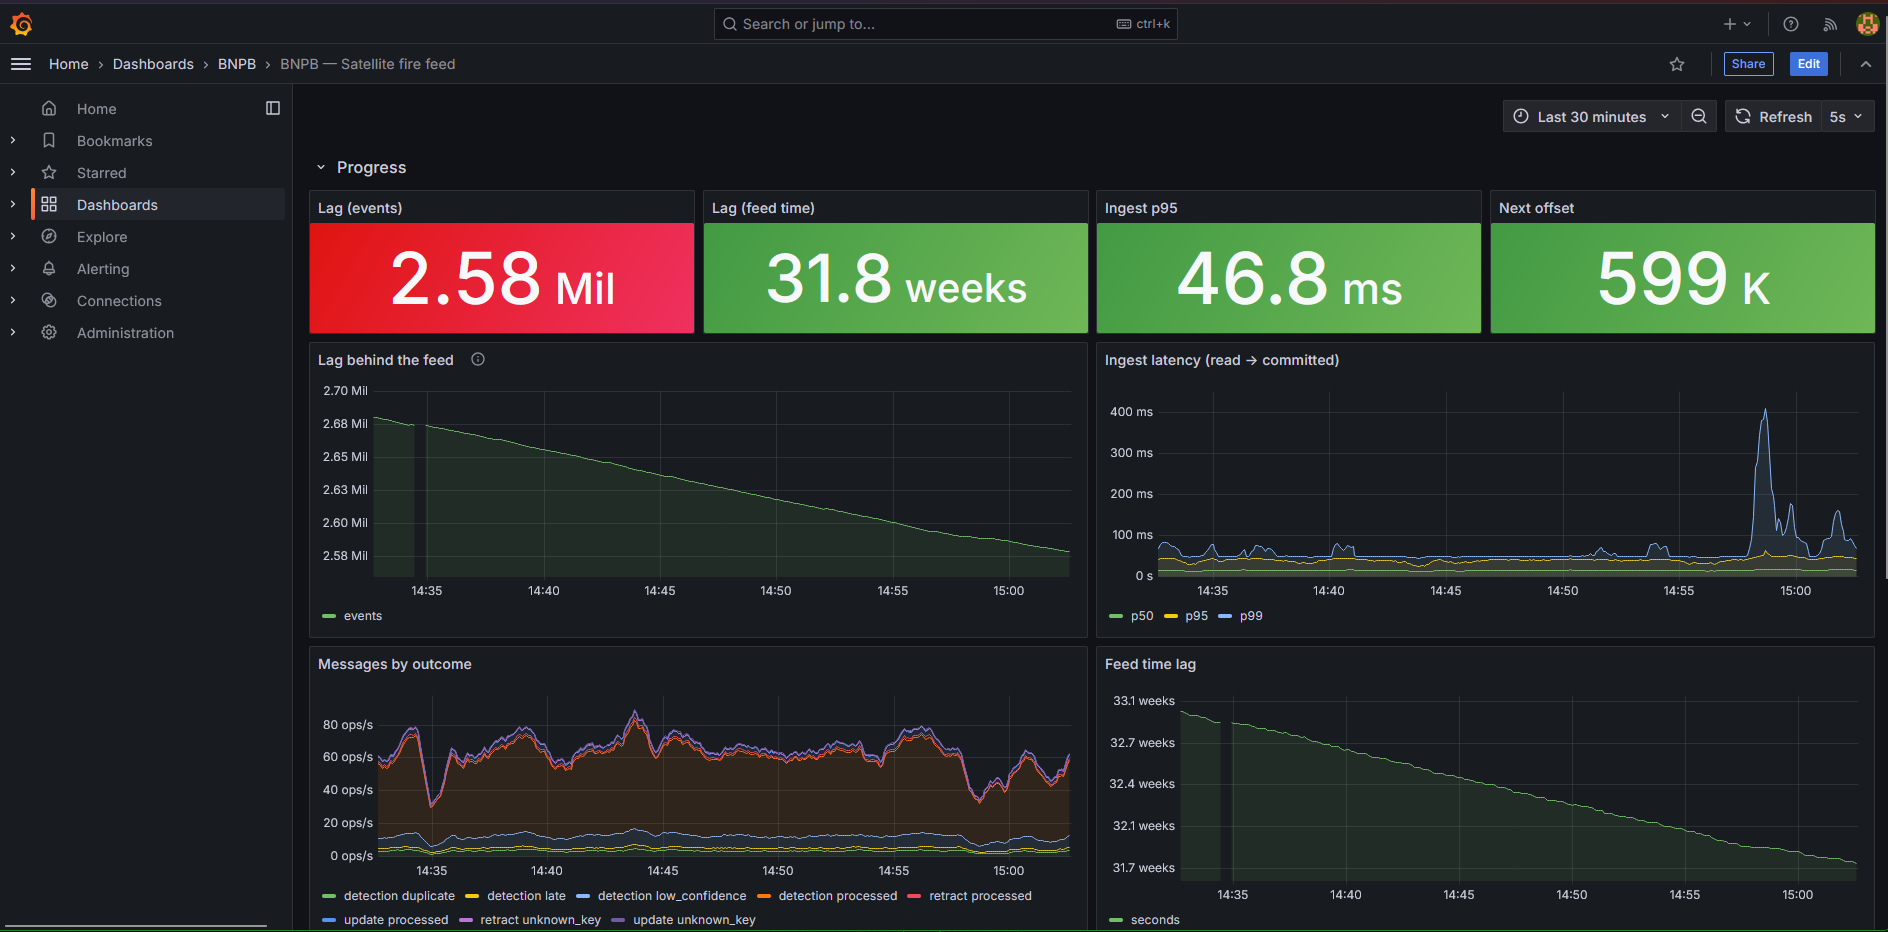
\includegraphics[width=\textwidth]{gambar/satellite-dashboard.png}
\caption{Dashboard \textit{Satellite fire feed} (Docker Compose, 30 menit). Lag $\pm$2,6 juta event berwarna merah karena ambang 1.000 event dibuat untuk keadaan normal. Kurvanya terus turun karena ingestor membaca lebih cepat daripada feed dan menghabiskan sisa \textit{backlog}. Latensi dari baca sampai komit p95 $\pm$47 ms.}
\label{fig:satellite-dashboard}
\end{figure}

\subsubsection{Jawaban atas Butir ``Di Laporan''}
\begin{enumerate}
\item \textbf{Persoalan:} kriteria 2 \textit{event time vs processing time}, \textit{watermark}, \textit{allowed lateness}. Kriteria 4 \textit{consumer lag / backpressure}. Kriteria 5 \textit{stateful processing} dengan \textit{atomic checkpoint} (\textit{exactly-once processing}).
\item \textbf{Pola M1:} \textit{polling} ditinggalkan untuk sumber ini dan diganti konsumsi aliran SSE dengan \textit{offset}. Pola M1 (\textit{polling} berkala dengan \textit{watermark} waktu) cocok untuk API yang hanya bisa ditanya. Feed satelit justru mendorong event berurutan dengan \textit{offset} yang dapat dilanjutkan, sehingga \textit{polling} hanya menambah jeda dan risiko celah. Jalur keluar memakai pola M1 yang sama: \textit{transactional outbox} lalu JetStream, kemudian Aggregator melakukan \textit{upsert} idempoten.
\item \textbf{Kapan kebakaran ``selesai dikenali'', keterlambatan, dan keadaan sementara:} kebakaran tidak ditutup pada jendela tetap. Setiap deteksi baru, \textit{update}, atau \textit{retract} memperbarui kebakaran yang bersangkutan dan dipublikasikan sebagai versi baru. Deteksi yang lebih tua 2 jam dari deteksi terbaru dihitung sebagai \textit{late}. Keadaan (deteksi, kebakaran, \textit{offset}, \textit{outbox}) tersimpan di \kode{satellite-store} dalam satu transaksi. Keadaan sementara terlihat oleh klien sebagai versi kebakaran yang terus bertambah (\kode{source\_version} naik). Klien selalu membaca versi terakhir dan tidak perlu menunggu kebakaran ``selesai''.
\item \textbf{Jaminan pemrosesan:} \textit{exactly-once} secara efektif: \textit{offset} dan keadaan dikomit atomik, \textit{outbox} + \kode{Nats-Msg-Id} + \textit{version guard} di Aggregator mencegah duplikat. Bukti: uji \textit{kill-and-restart} pada kriteria 5.
\end{enumerate}

\subsection{Problem 5: Pelampung yang Berbohong}

\subsubsection{Identifikasi Masalah}

\begin{longtable}{|p{1.6cm}|p{5.6cm}|p{7.7cm}|}
\hline
\textbf{Kriteria} & \textbf{Persoalan} & \textbf{Konsep dalam literatur}\\ \hline \endhead
2 & Sumber mengirim data yang salah, kedaluwarsa, ganda, atau berkualitas rendah sambil mengaku sehat & \textit{Input validation}, \textit{data quality}, \textit{quarantine / dead letter}, \textit{faulty (Byzantine-ish) source}, \textit{idempotent consumer}\\ \hline
3 & Satu sumber yang sakit menghabiskan sumber daya dan menyeret sumber lain & \textit{Cascading failure}, \textit{bulkhead}, \textit{timeout} (Nygard, \textit{Release It!})\\ \hline
4 & Permintaan ke sumber sakit terus diulang dan memperparah keadaan. Client menunggu hingga \textit{timeout} & \textit{Circuit breaker}, \textit{exponential backoff with jitter}, \textit{fail fast}, \textit{graceful degradation / serve stale}\\ \hline
5 & Kapasitas habis dan semua client dilayani sama buruknya & \textit{Load shedding}, \textit{prioritization / admission control} (Google SRE Book, ``Handling Overload'')\\ \hline
1, 8 & Peringatan kritis harus sampai dalam batas waktu & \textit{Priority lane}, SLI/SLO/\textit{error budget} (Google SRE Book)\\ \hline
\end{longtable}

\subsubsection{Rancangan Solusi}

Image Sensor Pantai berjalan tanpa modifikasi dari contoh manifest asisten (\kode{deploy/k8s/base/sensor/}). Satu-satunya komponen yang memanggil sensor adalah \kode{sensor-pantai-poller}:

\begin{lstlisting}
sensor-pantai --HTTP (pool sendiri, timeout 2 s, breaker)--> sensor-pantai-poller
   -> validasi tiap item
   -> kritis lebih dulu: BNPB_ALERTS -> notification-consumer (durable terpisah) -> penerima Tim Lapangan
   -> hazard.ingest.SENSOR_PANTAI op=upsert (COASTAL) -> Aggregator -> canonical store
   -> hazard.ingest.SENSOR_PANTAI op=reject (+alasan, payload mentah) -> dead_letters
\end{lstlisting}

\begin{longtable}{|p{3.4cm}|p{6.4cm}|p{5.1cm}|}
\hline
\textbf{Mekanisme} & \textbf{Konfigurasi} & \textbf{Alasan nilai}\\ \hline \endhead
\textit{Bulkhead} & Proses terpisah dengan \textit{pool} koneksi sendiri (maks 2) dan koneksi NATS sendiri. Aggregator tidak pernah memanggil sensor & Sensor lambat tidak dapat menghabiskan \textit{worker} atau koneksi BMKG/PVMBG\\ \hline
\textit{Timeout} & 2 s per permintaan & Respons normal p95 $\approx$ 0,3 s, tetapi sensor kadang lambat hingga 7,9 s\\ \hline
\textit{Circuit breaker} & Terbuka setelah 3 kegagalan berturut-turut. Terbuka 5 s, berlipat sampai 30 s, \textit{jitter} $\pm$20\%. \textit{half-open} mengizinkan 1 \textit{probe} & 3 kegagalan membedakan error sesaat dari gangguan. Batas 30 s menjaga pemulihan $\le$ 30 s setelah sensor pulih. \textit{Jitter} mencegah \textit{probe} serentak\\ \hline
\textit{Retry} & 0,5 s berlipat sampai 8 s, \textit{full jitter} 50--100\%, selama \textit{breaker} tertutup & Error sesaat (503 sporadis) dicoba ulang cepat tanpa badai \textit{retry}\\ \hline
Validasi kontrak & Field/tipe wajib, \kode{station\_id} dikenal, \kode{observed\_at} $\le$ 2 jam lebih tua dan $\le$ 1 menit lebih baru dari \kode{generated\_at} sensor, $|$anomali$|$ $\le$ 15 m, gelombang 0--30 m, \kode{quality = "ok"} & Waktu dibandingkan dengan jam sensor (60$\times$). 2 jam sensor $\approx$ 2 menit nyata, cukup untuk \textit{restart} poller tanpa menolak \textit{backlog} sah\\ \hline
Data ditolak & \kode{op=reject} ke \kode{dead\_letters} (\kode{parked}, alasan, payload mentah) ke \kode{/internal/audit/unprocessed} & Disisihkan dengan alasan, tidak pernah menjadi HazardEvent\\ \hline
Dedup & Kunci \kode{observation\_id@observed\_at} (per halaman + 50.000 kunci terakhir) dan \kode{Nats-Msg-Id} & Sensor mengirim ulang item. Setelah sensor \textit{restart}, ID dapat dipakai ulang\\ \hline
Jalur prioritas & Stream \kode{BNPB\_ALERTS} + durable consumer terpisah. Alert dipublikasikan paling awal. \textit{Redelivery} tanpa batas. \kode{EventID} = \kode{hazard\_id} kanonik & Alert tidak antre di belakang event biasa dan tidak dikirim dua kali oleh jalur reguler\\ \hline
Degradasi terkendali & \kode{meta.sources.sensor\_pantai} (UP/DEGRADED/OUTAGE/DOWN, \kode{last\_synced\_at}, \kode{stale\_since}) dari JetStream KV (cache 1 s) & Client langsung mendapat data terakhir + status. Client-api tidak menunggu sensor\\ \hline
Sensor diam / jam beku & DEGRADED bila observasi terbaru tertinggal $>$ 10 menit dari jam sensor. Gagal bila \kode{generated\_at} tidak bergerak 15 s & Sensor kadang menjawab 200 tanpa data baru\\ \hline
Sensor \textit{restart} & Cursor disimpan bersama jam sensor. Jam mundur atau cursor ditolak (4xx) membuat poller membaca dari awal & \kode{emptyDir} membuat data sensor mulai ulang saat pod dihapus\\ \hline
\textit{Load shedding} & \kode{MAX\_INFLIGHT} = 256 per pod client-api. Media maks 60\%, Tim Lapangan/Ops 100\%. 503 + \kode{Retry-After: 1} tanpa antrean & Kapasitas cadangan 40\% untuk Tim Lapangan. \isi{nilai final setelah \textit{tuning} di klaster demo}\\ \hline
Kondisi stasiun & 1 HazardEvent per stasiun, diperbarui saat \textit{severity} berubah atau tiap 5 menit waktu sensor. AWAS bila kritis, SIAGA $\ge$ 1,0 m / 4,0 m, WASPADA $\ge$ 0,5 m / 2,5 m & Laju tulis turun dari $\approx$ 4/s menjadi $<$ 1/s. Observasi kritis tetap mendapat HazardEvent AWAS sendiri\\ \hline
\end{longtable}

\subsubsection{Alasan Keputusan}
\begin{itemize}
\item \textbf{Poller di proses terpisah vs di dalam Aggregator:} siklus \textit{polling} Aggregator dipakai bersama oleh BMKG dan PVMBG, sehingga sensor yang lambat akan menunda sumber lain. Proses terpisah memberi isolasi penuh. Poller dijalankan 1 replika (\textit{Recreate}). Bila sempat ada dua (misalnya saat partisi), \textit{message ID} dan \textit{version guard} membuat publikasi ganda tidak berbahaya.
\item \textbf{\textit{Breaker} berbasis kegagalan berturut-turut vs rasio error:} poller hanya mengirim $\pm$1 permintaan/s, terlalu sedikit untuk jendela rasio yang stabil.
\item \textbf{Stream prioritas terpisah vs prioritas di satu stream:} JetStream tidak mendukung prioritas dalam satu stream. Stream dan consumer terpisah lebih sederhana dan terbukti.
\item \textbf{\textit{Shedding} berbasis \textit{in-flight} vs \textit{rate limit}:} \textit{rate limit} membatasi laju per client tanpa melihat beban sistem. \textit{in-flight} langsung mencerminkan kelambatan sistem.
\end{itemize}

\subsubsection{Batasan yang Disadari}
\begin{itemize}
\item Observasi kritis yang juga berkualitas \kode{suspect} ditolak (kontrak diutamakan) dan tercatat dengan alasannya. \isi{konfirmasi kebijakan oleh tim}
\item \textit{Backlog} yang lebih tua dari 2 jam waktu sensor (misalnya poller mati lama) ditolak sebagai \kode{expired}.
\item \textit{Load shedding} hanya melindungi client-api. Permintaan yang diterima tetap membebani Aggregator, sehingga \kode{MAX\_INFLIGHT} disetel sesuai kapasitas Aggregator.
\end{itemize}

\subsubsection{Bukti Penyelesaian}

\begin{longtable}{|p{3.4cm}|p{6cm}|p{5.5cm}|}
\hline
\textbf{Kriteria} & \textbf{Klaster pengembangan} & \textbf{Klaster demo}\\ \hline \endhead
1. 0 alert hilang, p95 $\le$ 5 s & Pod sensor dihapus, \textit{restart} terdeteksi 4 s, dan 3/3 alert sampai, rata-rata 13 ms dari deteksi ke penerima & Pod sensor dihapus pukul 09:33:50 UTC. \textit{Restart} terdeteksi 41 s kemudian (pod baru butuh $\pm$40 s untuk siap di VM). Ketiga alert kritis (\kode{obs-000120}, \kode{obs-000362}, \kode{obs-000601}) sampai ke penerima Tim Lapangan. Histogram \kode{notification\_delivery\_latency\_seconds\{path="priority"\}}: 3 dari 3 $\le$ 1 s (total 1,52 s, rata-rata 0,51 s), sehingga p95 $\le$ 1 s dan SLI 100\%. Dari log, jarak deteksi poller sampai diterima stub-sink 0,49 s, 12 ms, dan 25 ms. Sebelum diukur, stream \kode{BNPB\_ALERTS} berisi tepat 3 pesan walaupun sensor sudah di-\textit{restart} 4 kali (tidak ada alert ganda). Karena profil \textit{practice} selalu mengulang 3 observasi kritis yang sama, keadaan dedup jalur alert dikosongkan dulu agar pengukuran setara deploy baru.\\ \hline
2. Data pelanggar disisihkan & \kode{/internal/audit/unprocessed?source=SENSOR\_PANTAI}: \kode{parked} dengan alasan \kode{quality\_not\_ok}, \kode{expired}. Tidak ada di \kode{/v1/events} & \isi{}\\ \hline
3. Sumber lain memenuhi latensi M1 & \isi{} & \isi{k6 BMKG-only p95 saat sensor bermasalah}\\ \hline
4. Permintaan tidak melonjak, cepat, pulih sendiri & Sensor mati 65 s dengan hanya 5 permintaan (\textit{probe} +4/+10/+20/+36/+66 s). \kode{/v1/events} 0,3 s dengan status OUTAGE. UP lagi 16 s setelah sensor siap & Sensor di-\textit{scale} 0 selama 74 s. \textit{Breaker} terbuka 1 s setelah kegagalan ketiga, dan selama gangguan hanya 7 permintaan yang dikirim ke sensor (3 di awal, lalu \textit{probe half-open} pada +8, +22, +42, dan +69 s dengan jeda berlipat). \kode{/v1/events} tetap HTTP 200 dalam 0,85--1,62 s dengan \kode{sensor\_pantai.status} OUTAGE (lambatnya berasal dari CockroachDB yang kekurangan CPU, bukan dari sensor). \textit{Breaker} menutup sendiri 24 s setelah pod sensor siap dan status kembali UP tanpa intervensi.\\ \hline
5. Tim Lapangan dilayani saat \textit{overload} & 300 VU Media + 10 VU Tim Lapangan, \kode{MAX\_INFLIGHT}=20: Media ditolak 98\%, Tim Lapangan terlayani 92,6\% (Aggregator di satu laptop menjadi \textit{bottleneck}) & \isi{\kode{scripts/demo/m2/load/shedding.sh}}\\ \hline
6. Kombinasi kegagalan & \kode{scripts/demo/m2/gameday/gameday.sh} & \isi{}\\ \hline
7. Penjelasan dari dashboard & Grafana BNPB (Coastal, Aggregator, Services), Jaeger & \isi{tangkapan layar saat \textit{game day}}\\ \hline
8. Target keandalan & Lihat butir ``Di Laporan'' & \isi{budget terpakai}\\ \hline
\end{longtable}

\gambarplaceholder{Dashboard ``BNPB --- Coastal sensor and alert SLO'' selama game day}{5cm}

\subsubsection{Jawaban atas Butir ``Di Laporan''}
\begin{enumerate}
\item \textbf{Persoalan kriteria 2--5:} lihat tabel identifikasi pada bagian a.
\item \textbf{Mekanisme, konfigurasi, dan alasan nilai:} lihat tabel pada bagian b. \textbf{SLO jalur peringatan Tim Lapangan:} 99\% alert kritis sampai ke penerima $\le$ 5 s sejak terdeteksi, per jendela 1 jam. SLI = alert terkirim $\le$ 5 s di jalur prioritas $\div$ alert yang dipublikasikan poller (dihitung sekali per alert. Alert yang tidak pernah sampai dihitung gagal). \textit{Error budget} tersisa = $1 - (1 - \mathrm{SLI})/0{,}01$, ditambah \textit{burn rate} 15 menit.
\item \textbf{Perilaku menyimpang Sensor Pantai} (ditemukan dengan merekam \kode{/v1/observations} dan \kode{/healthz} setiap detik selama $\pm$17 menit $\approx$ 17 jam waktu sensor, profil \textit{practice}):
\begin{center}
\begin{tabularx}{\textwidth}{|X|X|}
\hline
\textbf{Perilaku} & \textbf{Penanganan}\\ \hline
\kode{/v1/observations} 503 ``sensor sedang tidak melayani'' padahal \kode{/healthz} 200. \kode{/healthz} sendiri kadang gagal & \kode{/healthz} tidak dipakai sebagai sinyal sehat. Kegagalan dihitung \textit{breaker}\\ \hline
Respons hingga 7,9 s & \textit{Timeout} 2 s, lalu \textit{retry/breaker}\\ \hline
Observasi identik dikirim ulang dalam satu halaman dan antar halaman & Dedup kunci + \textit{message ID}\\ \hline
\kode{quality: "suspect"} ($\pm$1,3\%) & Ditolak (\kode{quality\_not\_ok})\\ \hline
Diam $\pm$70 menit sensor, lalu banjir 18--200 item & Cursor + batas halaman per siklus. Status DEGRADED saat diam\\ \hline
Data mulai ulang dari 00:00 saat pod dihapus & Deteksi jam mundur, lalu baca dari awal\\ \hline
Jam sensor sendiri (60$\times$) & Semua aturan waktu memakai \kode{generated\_at}\\ \hline
\isi{perilaku tambahan dari profil \textit{exam}} & \\ \hline
\end{tabularx}
\end{center}
\item \textbf{Post-mortem \textit{game day}:}
\begin{itemize}
\item \textbf{Ringkasan:} kegagalan disuntikkan pada t=30 s (PVMBG \textit{outage}), t=60 s (pod sensor dihapus), t=90--150 s (partisi jaringan ke sensor), \isi{t=120 s skenario Tester Agent}, PVMBG pulih t=180 s, lalu jendela pemulihan tanpa intervensi. \isi{waktu pulih}
\item \textbf{Deteksi:} \isi{panel \textit{breaker} OPEN, \kode{sensor\_pantai.status} OUTAGE, sumber PVMBG OUTAGE, \kode{client\_api\_shed\_total}. Waktu deteksi}
\item \textbf{Dampak:} \isi{alert terlambat/hilang, Tim Lapangan terlayani (\%), Media ditolak (\%), \textit{error budget} terpakai (\%)}
\item \textbf{Mitigasi otomatis:} \textit{breaker} membatasi permintaan ke sensor. Data terakhir disajikan dengan status. Media di-\textit{shed}. PVMBG dilayani dari data terakhir. Sensor \textit{restart} ditangani dengan membaca dari awal.
\item \textbf{Perbaikan:} \isi{berdasarkan temuan, misalnya \textit{tuning} \kode{MAX\_INFLIGHT}, batas \textit{breaker}, kapasitas Aggregator}
\item \textbf{Timeline:} \isi{salin \kode{evidence/gameday/<run>/timeline.txt}}
\end{itemize}
\end{enumerate}


% ════════════════════════════ REFERENSI ═════════════════════════
\bagian{REFERENSI}

\begin{list}{}{\leftmargin=1.2cm \itemindent=-1.2cm \itemsep=6pt}
\item Akidau, T., Bradshaw, R., Chambers, C., Chernyak, S., Fernández-Moctezuma, R. J., Lax, R., McVeety, S., Mills, D., Perry, F., Schmidt, E., \& Whittle, S. (2015). The Dataflow Model: A practical approach to balancing correctness, latency, and cost in massive-scale, unbounded, out-of-order data processing. \textit{Proceedings of the VLDB Endowment, 8}(12), 1792--1803.
\item Akidau, T., Chernyak, S., \& Lax, R. (2018). \textit{Streaming Systems}. O'Reilly Media.
\item Beyer, B., Jones, C., Petoff, J., \& Murphy, N. R. (Eds.). (2016). \textit{Site Reliability Engineering: How Google Runs Production Systems}. O'Reilly Media. Bab ``Service Level Objectives'' dan ``Handling Overload''.
\item Brooker, M. (2015). \textit{Exponential backoff and jitter}. AWS Architecture Blog. \url{https://aws.amazon.com/blogs/architecture/exponential-backoff-and-jitter/}
\item Cockroach Labs. (n.d.). \textit{CockroachDB documentation: Replication layer, Multi-active availability, Configure replication zones}. \url{https://www.cockroachlabs.com/docs/v24.1/}
\item Fox, A., \& Brewer, E. A. (1999). Harvest, yield, and scalable tolerant systems. \textit{Proceedings of the Seventh Workshop on Hot Topics in Operating Systems (HotOS-VII)}, 174--178.
\item Google. (n.d.). \textit{Distroless}. GitHub. \url{https://github.com/GoogleContainerTools/distroless}
\item Go Authors. (n.d.). \textit{The Go programming language specification}. \url{https://go.dev/ref/spec}
\item Grafana Labs. (n.d.). \textit{Using k6}. \url{https://grafana.com/docs/k6/latest/}
\item Hohpe, G., \& Woolf, B. (2003). \textit{Enterprise Integration Patterns}. Addison-Wesley. (\textit{Dead Letter Channel}, \textit{Guaranteed Delivery}, \textit{Idempotent Receiver}).
\item Kleppmann, M. (2016). \textit{How to do distributed locking}. Martin Kleppmann's Blog. \url{https://martin.kleppmann.com/2016/02/08/how-to-do-distributed-locking.html}
\item Kleppmann, M. (2017). \textit{Designing Data-Intensive Applications}. O'Reilly Media. (Bab 6 \textit{Partitioning}, Bab 8 \textit{The Trouble with Distributed Systems}, Bab 11 \textit{Stream Processing}).
\item Kubernetes Authors. (n.d.). \textit{Kubernetes documentation: Deployments, StatefulSets, Network Policies, Configure Liveness and Readiness Probes}. \url{https://kubernetes.io/docs/}
\item NATS Authors. (n.d.). \textit{JetStream}. \url{https://docs.nats.io/nats-concepts/jetstream}
\item Nygard, M. T. (2018). \textit{Release It! Design and Deploy Production-Ready Software} (2nd ed.). Pragmatic Bookshelf. (\textit{Circuit Breaker}, \textit{Bulkheads}, \textit{Timeouts}, \textit{Shed Load}).
\item Ongaro, D., \& Ousterhout, J. (2014). In search of an understandable consensus algorithm. \textit{Proceedings of the 2014 USENIX Annual Technical Conference (USENIX ATC '14)}, 305--319.
\item OpenTelemetry Authors. (n.d.). \textit{OpenTelemetry Go documentation}. \url{https://opentelemetry.io/docs/languages/go/}
\item Prometheus Authors. (n.d.). \textit{Prometheus documentation: kubernetes\_sd\_config, Histograms and summaries}. \url{https://prometheus.io/docs/}
\item rs. (n.d.). \textit{Zerolog: Zero allocation JSON logger}. GitHub. \url{https://github.com/rs/zerolog}
\item SUSE / Rancher. (n.d.). \textit{K3s documentation}. \url{https://docs.k3s.io/}
\item The Go Authors. (n.d.). \textit{Go package bbolt}. \url{https://pkg.go.dev/go.etcd.io/bbolt}
\item NASA FIRMS. (n.d.). \textit{VIIRS (S-NPP, NOAA-20, NOAA-21) 375 m Active Fire product: attributes and confidence}. \url{https://www.earthdata.nasa.gov/data/instruments/viirs}
\item Richardson, C. (n.d.). \textit{Pattern: Transactional outbox}. microservices.io. \url{https://microservices.io/patterns/data/transactional-outbox.html}
\item W3C. (2021). \textit{Trace Context} (W3C Recommendation). \url{https://www.w3.org/TR/trace-context/}
\item WHATWG. (n.d.). \textit{HTML Living Standard: Server-sent events}. \url{https://html.spec.whatwg.org/multipage/server-sent-events.html}
\end{list}


\end{document}
